\documentclass[phd,bottom,nosig]{usbthesis}
%\includeonly{chapter1}
\bibliographystyle{apj}
\usepackage{graphicx}
\usepackage{color}
\usepackage{bm}
\usepackage{amsmath}
\usepackage{amssymb}
%\usepackage{cleveref}
\usepackage{setspace}
\usepackage{array}
\usepackage{tabularx}
\usepackage{multirow}
\usepackage{afterpage}
\usepackage{dirtytalk}
\usepackage{hhline}
\usepackage{url}
\usepackage{verbatim}
\usepackage{pdfpages}
\usepackage{hyperref} % see the file hyperref.cfg for options
\usepackage[T1]{fontenc}
%\usepackage{indentfirst} % I find it ugly if the first paragraph is indented
\usepackage{footmisc} % provides \footref and \mpfootnotemark commands
\usepackage{xspace}
\usepackage{natbib}
%\usepackage[nottoc]{tocbibind}
%Make caption labels bold
\usepackage[labelfont=bf]{caption}

%Edit graphics path?
%\graphicspath{{./}{C://Users//Nathan//Pictures/}}


%\sloppy

% Math definitions
%\input{mathdefs}

% Latin abbreviations
\providecommand*{\eg}{\emph{e.\,g.}\xspace}%
\providecommand*{\ie}{\emph{i.\,e.}\xspace}%

%CREF CITATION COMMAND
\newcommand{\crefrangeconjunction}{--}
\newcommand{\micron}{$\mu m$}
\newcommand{\file}{}
\newcommand{\aj}{AJ}			% Astronomical Journal
\newcommand{\araa}{ARA\&A}		% Annual Review of Astron and Astrophys
\newcommand{\apj}{ApJ}			% Astrophysical Journal
\newcommand{\apjl}{ApJLett}		% Astrophysical Journal, Letters
\newcommand{\apjlett}{ApJLett}		% Astrophysical Journal, Letters
\newcommand{\apjs}{ApJS}		% Astrophysical Journal, Supplement
\newcommand{\apjsupp}{ApJS}		% Astrophysical Journal, Supplement
\newcommand{\ao}{Appl.~Opt.}		% Applied Optics
\newcommand{\apss}{Ap\&SS}		% Astrophysics and Space Science
\newcommand{\aap}{A\&A}			% Astronomy and Astrophysics
\newcommand{\astap}{A\&A}		% Astronomy and Astrophysics
\newcommand{\aapr}{A\&A~Rev.}		% Astronomy and Astrophysics Reviews
\newcommand{\aaps}{A\&AS}		% Astronomy and Astrophysics, Supplement
\newcommand{\azh}{AZh}			% Astronomicheskii Zhurnal
\newcommand{\baas}{BAAS}		% Bulletin of the AAS
\newcommand{\jrasc}{JRASC}		% Journal of the RAS of Canada
\newcommand{\memras}{MmRAS}		% Memoirs of the RAS
\newcommand{\mnras}{MNRAS}		% Monthly Notices of the RAS
\newcommand{\pra}{Phys.~Rev.~A}		% Physical Review A: General Physics
\newcommand{\prb}{Phys.~Rev.~B}		% Physical Review B: Solid State
\newcommand{\prc}{Phys.~Rev.~C}		% Physical Review C
\newcommand{\prd}{Phys.~Rev.~D}		% Physical Review D
\newcommand{\pre}{Phys.~Rev.~E}		% Physical Review E
\newcommand{\prl}{Phys.~Rev.~Lett.}	% Physical Review Letters
\newcommand{\pasp}{PASP}		% Publications of the ASP
\newcommand{\pasj}{PASJ}		% Publications of the ASJ
\newcommand{\pasa}{PASA}   % Publications of the Astronomical Society of Australia
\newcommand{\qjras}{QJRAS}		% Quarterly Journal of the RAS
\newcommand{\revmodphys}{Rev.\ Mod.\ Phys.} %Rev Mod Phys
\newcommand{\skytel}{S\&T}		% Sky and Telescope
\newcommand{\solphys}{Sol.~Phys.}	% Solar Physics
\newcommand{\sovast}{Soviet~Ast.}	% Soviet Astronomy
\newcommand{\ssr}{Space~Sci.~Rev.}	% Space Science Reviews
\newcommand{\zap}{ZAp}			% Zeitschrift fuer Astrophysik
\newcommand{\nat}{Nature}		% Nature
\newcommand{\iaucirc}{IAU~Circ.}       	% IAU Circulars
\newcommand{\aplett}{Astrophys.~Lett.} 	% Astrophysics Letters
\newcommand{\apspr}{Astrophys.~Space~Phys.~Res.}% Astrophysics Space tPhysics Research
\newcommand{\fcp}{Fund.~Cosmic~Phys.}  % Fundamental Cosmic Physics
\newcommand{\gca}{Geochim.~Cosmochim.~Acta}   % Geochimica Cosmochimica Acta
\newcommand{\grl}{Geophys.~Res.~Lett.} % Geophysics Research Letters
\newcommand{\jcp}{J.~Chem.~Phys.}	% Journal of Chemical Physics
\newcommand{\jgr}{J.~Geophys.~Res.}	% Journal of Geophysics Research
\newcommand{\nphysa}{Nucl.~Phys.~A}   % Nuclear Physics A
\newcommand{\physrep}{Phys.~Rep.}   % Physics Reports
\newcommand{\physscr}{Phys.~Scr}   % Physica Scripta
\newcommand{\planss}{Planet.~Space~Sci.}   % Planetary Space Science
\newcommand{\procspie}{Proc.~SPIE}   % Proceedings of the SPIE
%\hyphenation{put words here which LaTeX does not hy-phen-ate
%pro-per-ly}


\author{Rahul Indrakant Patel}%
\title{Carefully Identifying Debris Disks with WISE}%

\month{????} \year{2015}%

\program{Physics}%

%\director{Axel Drees}{Professor, Department of Physics and Astronomy}%
%\chairman{Peter Stephens}{Professor, Department of Physics and Astronomy}%
%\fstmember{Stephen Peggs}{Professor, Department of Physics and Astronomy}%
%\2ndmember{Mike Zingale}{Professor, Department of Physics and Astronomy}%
%\outmember{Igor Pogorelsky}{Physicist}{Brookhaven National Laboratory}%
%\outmember{Brian Sheehy}{Physicist}{Brookhaven National Laboratory}%
%\dean{Charles Taber}%


\begin{document}

\singlespacing %
\pagenumbering{roman} %

\maketitle %
%\makeapproval %


\newpage
\pagenumbering{gobble}

\vspace*{32\baselineskip}
\vspace*{1\baselineskip}
\centerline{Copyright by}
\centerline{Rahul Indrakant Patel}
\centerline{2015}


\newpage
\pagenumbering{roman}
\setcounter{page}{2}

%Add committee page
\centerline{\bf{Stony Brook University}}
\vspace*{1\baselineskip}
\centerline{The Graduate School}
\vspace*{2\baselineskip}
\centerline{Rahul Indrakant Patel}
\vspace*{2\baselineskip}
\centerline{We, the dissertation committee for the above candidate for the}
\vspace*{1\baselineskip}
\centerline{Doctor of Philosophy degree, hereby recommend}
\vspace*{1\baselineskip}
\centerline{acceptance of this dissertation}
\vspace*{2\baselineskip}
\centerline{\bf{Stanimir Metchev - Dissertation Advisor}}
\centerline{\bf{Professor, Department of Physics and Astronomy}}
\vspace*{1\baselineskip}
\centerline{\bf{Michael Zingale - Chairperson of Defense}}
\centerline{\bf{Professor, Department of Physics and Astronomy}}
\vspace*{1\baselineskip}
\centerline{\bf{Matthew Dawber - Committee Member}}
\centerline{\bf{Professor, Department of Physics and Astronomy}}
\vspace*{1\baselineskip}
\centerline{\bf{Rebecca Oppenheimer - Committee Member}}
\centerline{\bf{Professor, American Museum of Natural History}}
\vspace*{2\baselineskip}
\centerline{This dissertation is accepted? by the Graduate School}
\vspace*{3\baselineskip}
\centerline{Charles Taber}
\centerline{Dean of the Graduate School}

\newpage

\begin{abstract}
    garble%\input{abstract}
\end{abstract}

\begin{dedication}
   Probably to a lot of people. \textbf{I was writing this part of my thesis when New Horizon's crossed Pluto earlier in the day.}
\end{dedication}

\tableofcontents %
\listoffigures %
\listoftables %

\begin{acknowledgements}

\end{acknowledgements}

\pagestyle{thesis}


%%%%%%%%%%%%%%%%%%%%%%%%%%%%%%%%%%%%%%%%%%%%%%%%%%%%%%%%%%%%%%%%%%%%%%%%%%%%%%%%

\newpage
\pagenumbering{arabic}

\chapter{Introduction} \label{chap:intro}
\section{Solar System Context}\label{sec:ch1_context}

    Since the discovery of the first extrasolar planets (exoplanet) around a main-sequence star, \citep[HD~114762~b and 51~Pegasi~b,][respectively]{Latham1989, Mayor1995}, a revolution has occurred in our understanding of planetary formation and evolution. We have seen exoplanets of a variety of flavors; gas giants at fractions of an astronomical unit (AU) from their star, binary planetary systems and even compact multi-planet systems. Giant planets are found with eccentricities ranging from 0--0.9, with sometimes large mutual inclinations. And roughly 50\% of solar type stars have a chance of hosting a compact multi-planet system with periods shorter than a year \citep[see review by][]{Winn2015}. 
    
    In contrast, the planets in our Solar System follow nearly circular, low inclination orbits at distances such that terrestrial and gas giants are separated by the snow-line (see \S~\ref{sec:solar_system}). Since this Solar System is the only one we know of where a planet can sustain life, perhaps the key to finding another is to search for systems with similar architecture. Of course there are a few exoplanetary systems that may seem architecturally similar to our own. The HR~8799 multi-planet system is the perfect example, where the system's four gas giant planets are at the same thermal radial distance from the HR~8799 star as our gas giants are to our Sun \citep{Marois2010}. 
    
    But this is one in a multitude of over a thousand planets we have uncovered. And if the majority of planets we are finding do not resemble the architecture of the Solar System, we have to ask: Is the existence of another habitable planet likely? If so, how can we identify a system that is hospitable to an Earth analog?
    %===================================================================
    %                DIVERSITY OF EXOPLANETS
    %===================================================================
    \begin{figure}
    \centering
    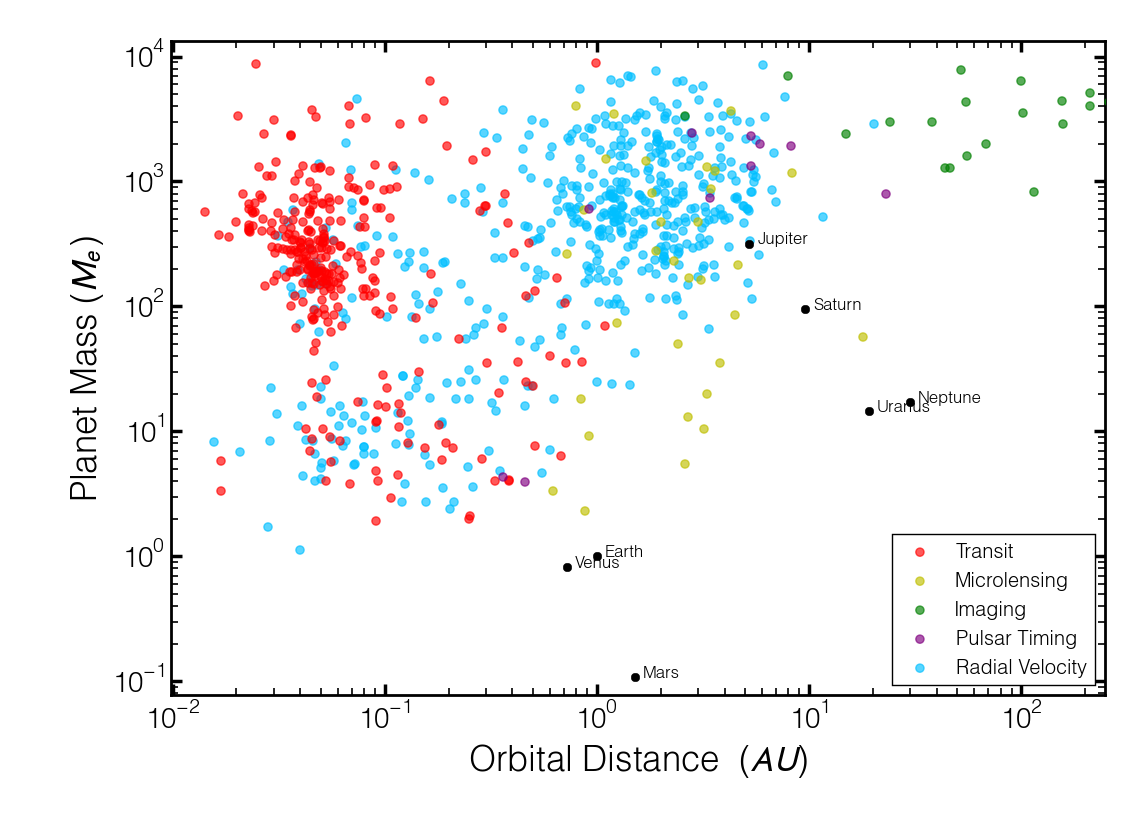
\includegraphics[width=\textwidth]{Ch1/exoplanet_detections_june2015} 
    \caption[Exoplanet Statistics]{Distribution of exoplanet masses vs. their estimated orbital distance and color coded based on the technique used to detect them. This plot only shows exoplanets detected as of June 2015.  Only planets with catalogued masses and orbital distances were plotted. $M \sin(i)$ values were used when exact values for the planet mass were unavailable. Solar System data is also plotted. Data was downloaded from \url{http://exoplanetarchive.ipac.caltech.edu/}.}
    \label{fig:known_exoplanets}
    \end{figure}
    %===================================================================
    
    We have seen over the last thirty years, that exoplanetary systems can also be identified by the presence of any dusty disks orbiting a main-sequence star. The first unresolved detection of extrasolar debris disks was by the \textit{Infrared Astronomical Satellite} (\iras) in 1983 of the Vega debris disk \citep{Aumann1984}. Further evidence from resolved images was taken by \citet{Smith1984} of the debris disks around the $\beta$~Pictoris system and galvanized the idea of these disks, which are created from the collisional grinding of planetesimals, are stirred by large planets  (see Figure~\ref{fig:smith_terrile_betapic}). Given that evidence exists that our own Solar System is a result of the concurrent evolution of our circumsolar disk and planets, then perhaps similarities can be drawn between what our circumsolar disk looked like at different stages in its evolution and the extrasolar debris disks astronomers have detected over the last thirty years. Another way to investigate this is to ask: is the likelihood of a system like ours --- and hence the possibility of life --- linked with the evolution of the disk and planets as a whole?
    
    This thesis takes a step toward investigating these questions by identifying additional systems which have previously been overlooked and may hold a wealth of information with which to place our Solar System in context. 
    
    %===================================================================
    %                SMITH TERRILE BETA PIC
    %===================================================================
    \begin{figure}
    \centering
    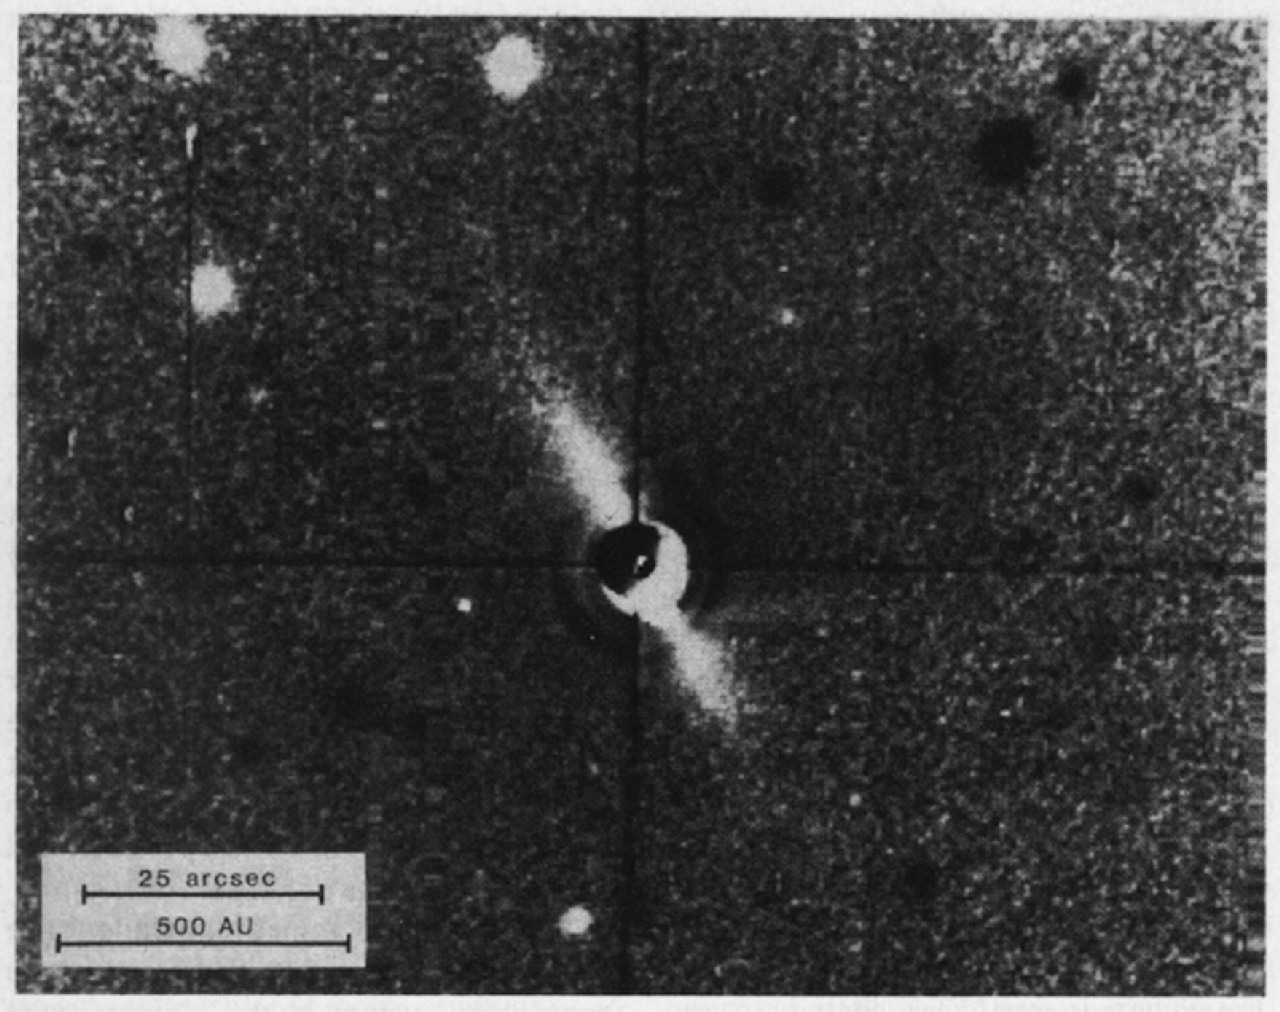
\includegraphics[width=.6\textwidth]{Ch1/betapic_SmithTerrile_84} 
    \caption[First Resolved Debris Disk: $\beta$~Pictoris]{Resolved disk emission around the $\beta$~Pictoris star. First ever resolved image of a debris disk. The image was taken using a coronagraph at the Las Campanas observatory in Chile. The disk is edge-on and composed of solid particles. As noted in \citet{Smith1984}, the flattened shape, rather than a spherical shell of particles is circumstantial evidence of planet formation. The circular shape in the center is due to the coronagraph and imperfect subtraction of the standard star.}
    \label{fig:smith_terrile_betapic}
    \end{figure}
    %===================================================================
    
    %Given that our own debris disk is created from the interplay between the planets and the minor bodies, studying debris disks can inform us of potentially undiscovered planetary systems, as well as help place our own Solar System in context. Thus, the next question to ask is whether nature can mimic a similar disk architecture such as ours and how we our system fits into the backdrop of the multitude of planetary system detections. 
    
    
\section{The Solar System's Debris Disk}\label{sec:ch1_ssdisk}

     \subsection{Current Configuration}
    
    The eight planets in the Solar System follow a relatively ordered configuration. With the exception of Mercury, the orbits are close to circular, and are closely inclined to the invariable plane, where inclination angles range from $0.33^{\circ}$--$2.19^{\circ}$. The four rocky planets are located interior to 1.7~AU, while the four gas giant planets are located beyond the snow-line --- the point in relation to the Sun beyond which volatile molecules (e.g., $H_2O, CH_4$) condense --- and all the way out to 30~AU. 
    
    The inner and outer planets are also segregated by a disk of material known as the Main Asteroid belt. Located between the orbit of Mars and Jupiter, the Asteroid belt is composed of over a million kilometer-sized objects that can be metallic, stony or even carbon rich in composition.
    
    It has been estimated that the mass of the Asteroid belt is $\sim0.04 M_{moon}$, a value that was much larger in the early Solar System (see \S~\ref{sec:solar_system}). Beyond the orbit of Neptune lies a large reservoir or minor planets composed of icy, volatile, cometary material with sizes greater than 1~km. These minor bodies, distributed in a thin belt the width of 20~AU, are known as the Edgeworth-Kuiper Belt (EKB).
    
    %===================================================================
    %                  THE SOLAR SYSTEM DIAGRAM
    %===================================================================
    \begin{figure}[!h]
    \centering
    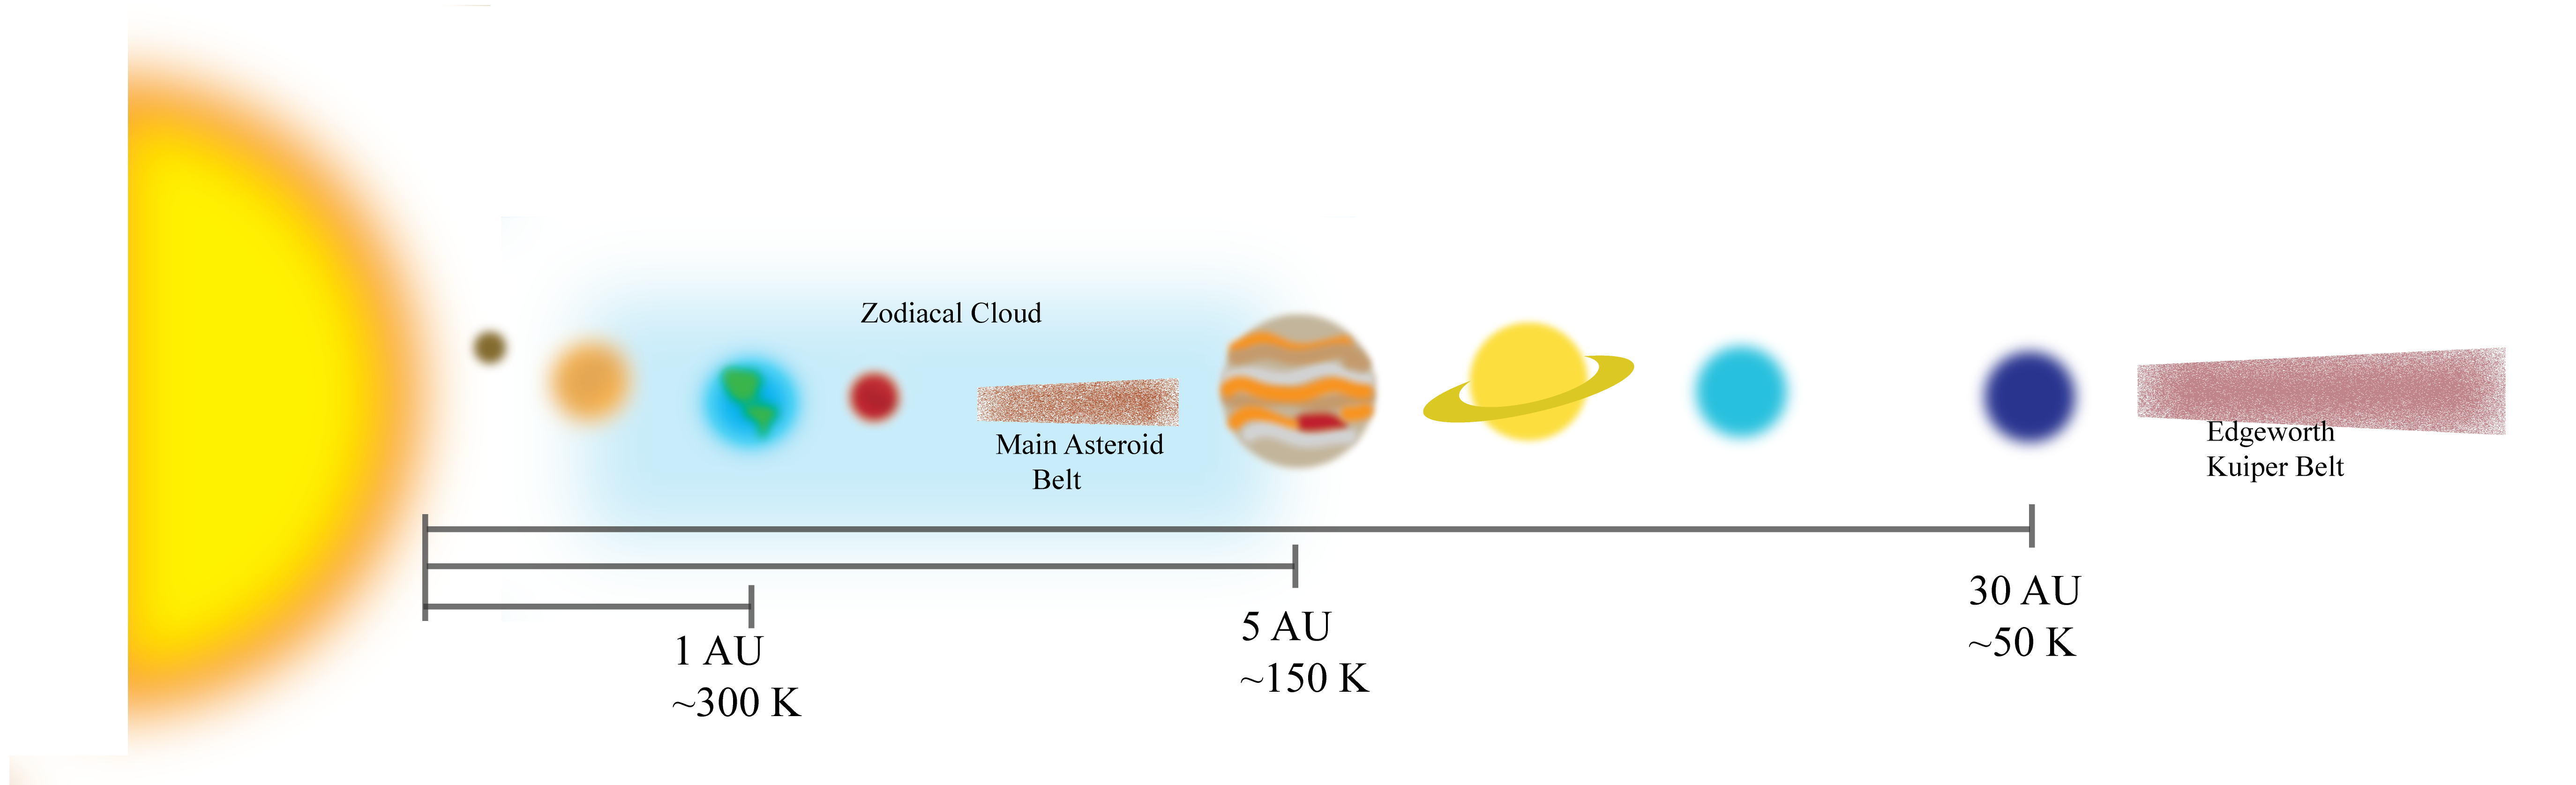
\includegraphics[width=\textwidth]{Ch1/SolarSystem_RPatel} 
    \caption{Caption}
    \label{fig:solar_system}
    \end{figure}
    %===================================================================
    
    
    
    %===================================================================
    %               THE Zodiacal Dust 
    %===================================================================
    \begin{figure}
    \centering
    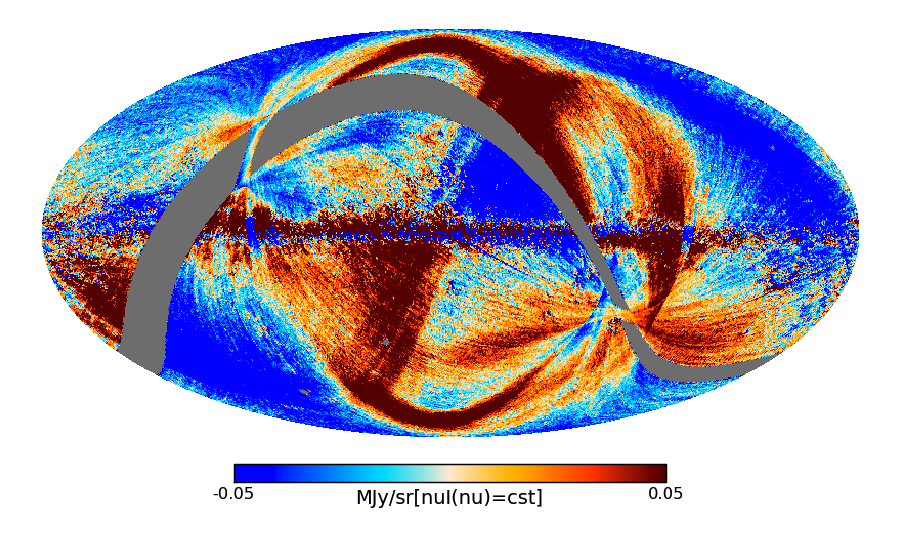
\includegraphics[width=.8\textwidth]{Ch1/zodiacal_planck} 
    \caption[Zodiacal Light Emission From Planck]{Galactic coordinate projection of the sky in the 850 GHz band from the Planck Satellite \citep{Ade2014}. The Zodiacal light emission is seen passing diagonally from the lower left to the top right, crossing the middle of the galactic plane. The top and bottom arcs are due to instrumental far side lobes.}
    \label{fig:ZD_Planck}
    \end{figure}
    
    
    
    
    \begin{figure}
    \centering
    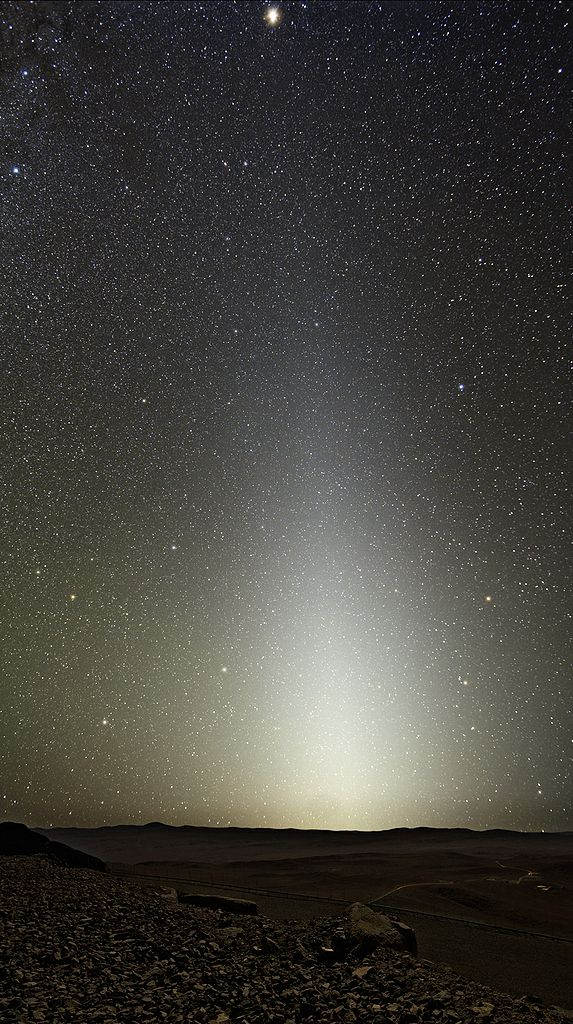
\includegraphics[width=0.25\textwidth]{Ch1/Zodiacal_Light_Paranal} 
    \caption[Zodiacal Light On Earth]{A faint glow seen along the ecliptic reveals the presence of 100\micron\  sized grains that comprise the Zodiacal Light. Image credit to the European Southern Observatory. Image was taken at Cerro Paranal, Chile \url{http://www.eso.org/public/unitedkingdom/images/zodiacal-light/}}
    \label{fig:ZD_ESO}
    \end{figure}
    %===================================================================
    
    
    In addition to the rings of large rocky bodies, a population of 10--100\micron\ sized cometary and silicate grains inhabits the Solar System. This disk, known as the Zodiacal Cloud, has been seen in scattered light observations \citep{Hahn2002}, thermal emission from the Planck \citep{Maris2006, Ade2014}, COBE \citep{Kelsall1998}, and the \iras\ \citep{Sykes1990} missions, as well as inferred from spacecraft impact experiments. From the ground, the Zodiacal Cloud can be seen only on the darkest of nights, as a faint glow along the ecliptic (see Figure~\ref{fig:ZD_ESO}). The inner Zodiacal Cloud extends from the orbit of Venus all the way out to Jupiter. From most recent studies, it is thought that mm--cm sized grains are ejected from Jupiter Family Comets (JFC) as they approach the large tidal forces of Jupiter's gravity. The smaller sub-mm sized grains, which comprise the disk are thought to be created from the grinding down of the larger mm--cm sized ejected grains. The overall mass of the inner Zodiacal Cloud has been estimated to be $\sim1-2\times10^{19}$~g \citep{Nesvorny2010}. The Zodiacal Cloud's density is so low that the overall disk brightness, when compared to the total emission of the Sun at all wavelengths (bolometric luminosity) is $L_{ZODY}/L_\odot \sim 2\times10^{-7}$ \citep{Nesvorny2010}. 


    
    \subsection{Dynamical Evolution Of Our Planetary System}\label{sec:solar_system}
    
    Beyond simply learning about the structure of the present-day Solar System, it is important to understand how the Solar System evolved into its present form. Although it is impossible to detail the entire history of the Solar System's evolution, it is important to understand that the current architecture of the Solar System would not be possible without the combined evolution of the planets as well as the remnant asteroidal and cometary disks. 
    
    It is generally accepted that all the planets formed within the first 100 Myr \citep[upper limit based on the final accretion time to create Earth;][]{Allegre2008}, after the Sun reached its place on the main-sequence. During this time, it has been hypothesized that the planets were in a compact configuration, all of them residing within 15~AU of the Sun \citep{Batygin2010}. Roughly 4.0--3.7~Gyr ago, scattering of the planetesimal populations that lay outside the orbit of Neptune at 15~AU resulted in angular momentum exchange between the gas giants and the disk. This led to a period of instability, in which Jupiter and Saturn's orbits diverged, and eventually crossed their mutual 1:2 mean motion resonance. From this, Jupiter migrated inward by $<0.5$~AU \citep{Morbidelli2010}, and pushed Saturn, Uranus and Neptune further out into the Solar System \citep{Tsiganis2005}. 
    
    This migration led to a period known as the Late Heavy Bombardment (LHB). During this time, Jupiter's short migration would have depleted the Asteroid belt by a factor or 10, and 97\% of the EKB was probably removed as a result of Neptune's outward migration. The scattered comets and asteroids during this period are most likely responsible for the Lunar craters we see today \citep{Gomes2005}. It is also thought that a fraction of Earth's water supply was transported during the LHB either from the EKB or from water rich asteroids. In addition, the depletion of the Asteroid belt by Jupiter has implications for the emergence of life on Earth, as a massive Asteroid belt today might have resulted in a higher frequency of Terrestrial impacts. In essence, the dynamical friction between the giant planets and the outer disk, which led to the migration of the outer planets, and consequentially the depletion of both the Asteroid belt and EKB, most likely laid the groundwork for life to flourish on Earth. Thus, it is these similar relationships a planetary system may have with its environment, and as such, influences its evolution, that we would like to investigate around other star systems. 

\section{Circumstellar Disk Evolution}
    
    Understanding the physical nature and processes governing the evolution of circumstellar disks is important if we are to understand the similarities between other systems and our own disk throughout its lifetime. In this section, I briefly outline the properties and characteristics of young gas-rich protoplanetary disks and their evolution into a dusty debris disk.

    \subsection{Protoplanetary Disk Evolution}
    
    The paradigm of planet formation begins with a nascent protoplanetary disk (PPD), composed of primordial gas and dust that remains post-star formation. The primordial material forms into a circumstellar disk, as a consequence of angular momentum conservation. The final radial extent of the disk is heavily sensitive to the angular rotation of the central star ($\Omega^2$) and even more sensitive to the infall time of the primordial material ($t_{infall}^3$) \citep{Terebey1984}. It is well accepted that 90--99\% of a PPD is composed of gas, while the rest is made of micron to mm sized dust grains.
    
    The bulk of the gas is comprised of neutral $H_2$. Though difficult to measure, mid-IR rotational lines have been observed from hot ($>600$~K) $H_2$ from the ground in systems like AB~Aurigae \citep{Bitner2007}. Typically, however, tracers such as $CO$, and $HCN$ line emissions are observed at sub-mm wavelengths to detect the gas in PPDs \citep[e.g., for stars in young associations such as Ophiuchus and Taurus-Auriga,][respectively]{Andre1994,Beckwith1990}. These observations have shown that the size of these disks can range from 10--100~AU, with masses $>0.005M_\odot$ \citep{Osterloh1995}. Dust masses are typically derived from dust thermal emission at mm-wavelengths, which probe the large grain population. The masses are typically derived by assuming an upper limit to the grain size (usually around mm sizes) and some assumed opacity values \citep{Beckwith1990}. Figure~\ref{fig:disk_masses} shows the masses of observed PPDs (ages $<10$~Myr), indicating disk masses on the order of a few hundred $M_{earth}$. 
    
    %===================================================================
    %   DISK MASSES FIG 3 WYATT 2008
    %===================================================================
    \begin{figure}
    \centering
    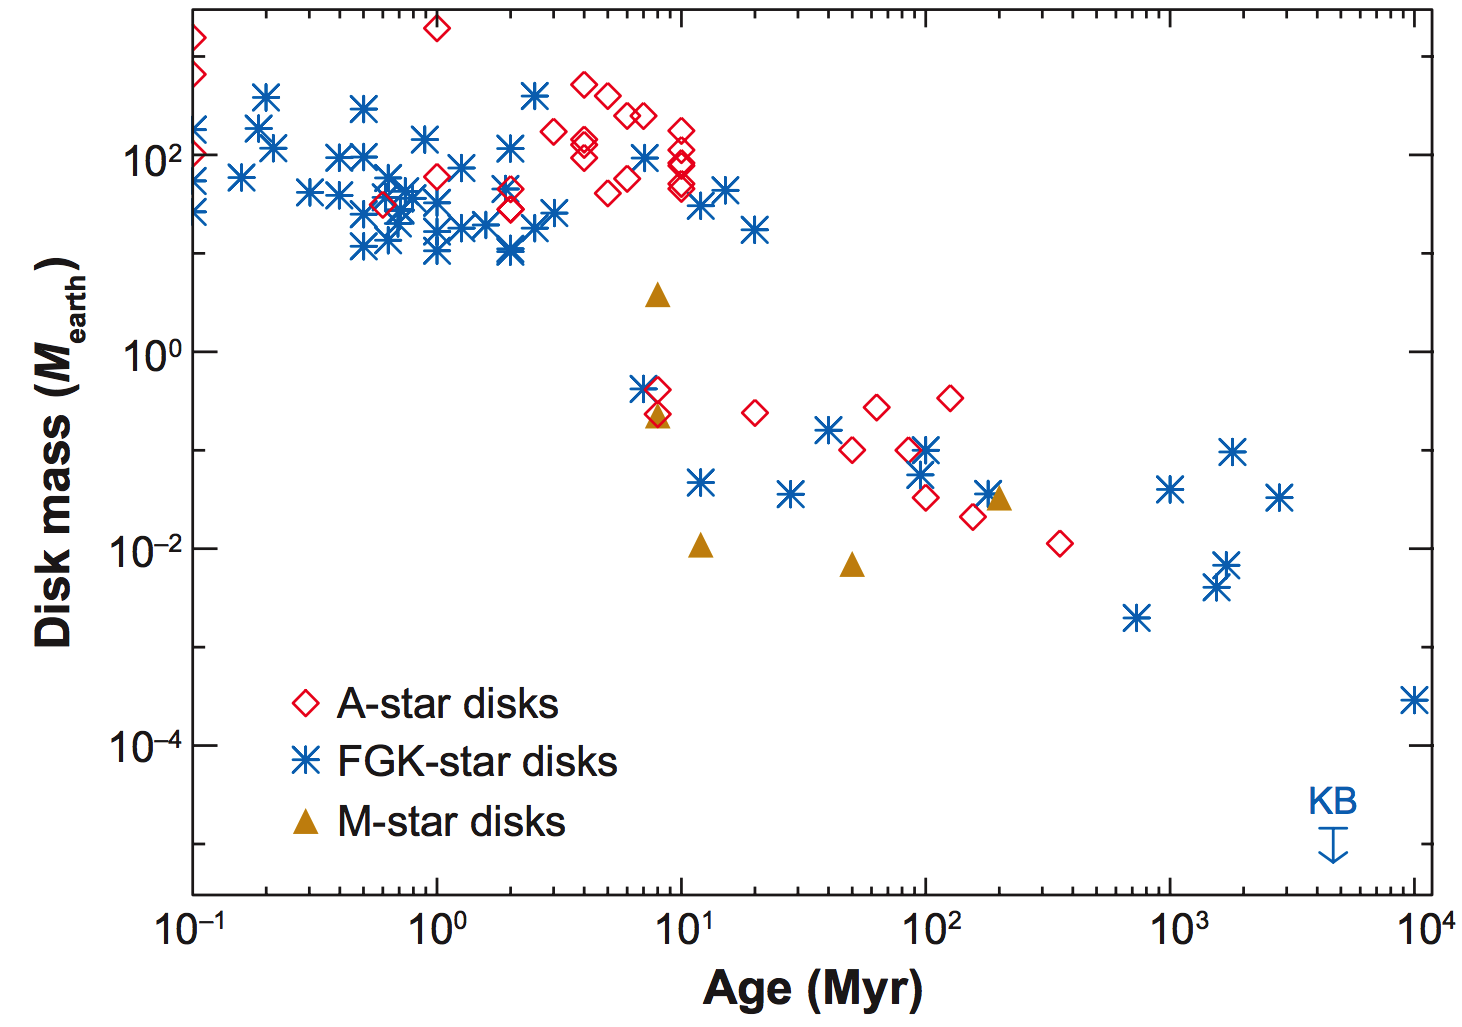
\includegraphics[width=.8\textwidth]{Ch1/diskmass_age_wyatt2008} 
    \caption[Protoplanetary and Debris Disk Masses Over Time]{Disk masses vs. age taken from \citet{Wyatt2008}. Disk masses were derived using sub-mm observations of disks. Different symbols represent different stellar masses (spectral types). The upper limit mass of the Kuiper Belt has also been plotted for contextual purposes.}
    \label{fig:disk_masses}
    \end{figure}
    %===================================================================
    
    The majority of the primordial gas and dust dissipates within the first $\sim$10~Myr. Viscous accretion of gas and dust onto the star has been attributed to the clearing of the inner regions (a few AU) of the star, which is supported by a lack of near-IR flux (2--5\micron) and the presence of forbidden line accretion signatures \citep[e.g., OI, SII][]{Hartigan1995}. Photoevaporation from the central star will also carve out the outer disk. In this process, high-energy UV and X-Ray photons can excite gas and dust molecules enough so that they are no longer bound to the system, and simply evaporate into interstellar space. The replenishment of material into the inner disk after the viscous accretion has halted, is inhibited from extreme-UV photons from the central star. The disk can also be dissipated via external sources. Usually, young stars are found in clusters with thousands of stars. A few of these will be O stars, that irradiate the surrounding environment in intense ionizing UV radiation \citep{Adams2004}. From this, mass loss of the disk will be expedited. 
    
    During this entire process, grain-growth becomes important, as it not only removes mass from the gas rich, but also provides the seeds for future planetary creation. Micron sized grains will typically feel a pressure gradient, since the gas rotates at sub-Keplerian speeds. As a result, grains will eventually collide, increase in mass and size, and be dragged to the mid-plane of the disk, where they can further grow to form the cores of giant planets, as well as asteroids and comets. The presence of any fully formed planets within this time can start sculpting the disk. Figure~\ref{fig:ppd_2_dd} illustrates these different processes.
    
    %===================================================================
    %   ILLUSTRATION OF EVOLUTION OF PPD TO DEBRIS DISK
    %===================================================================
    \begin{figure}
    \centering
    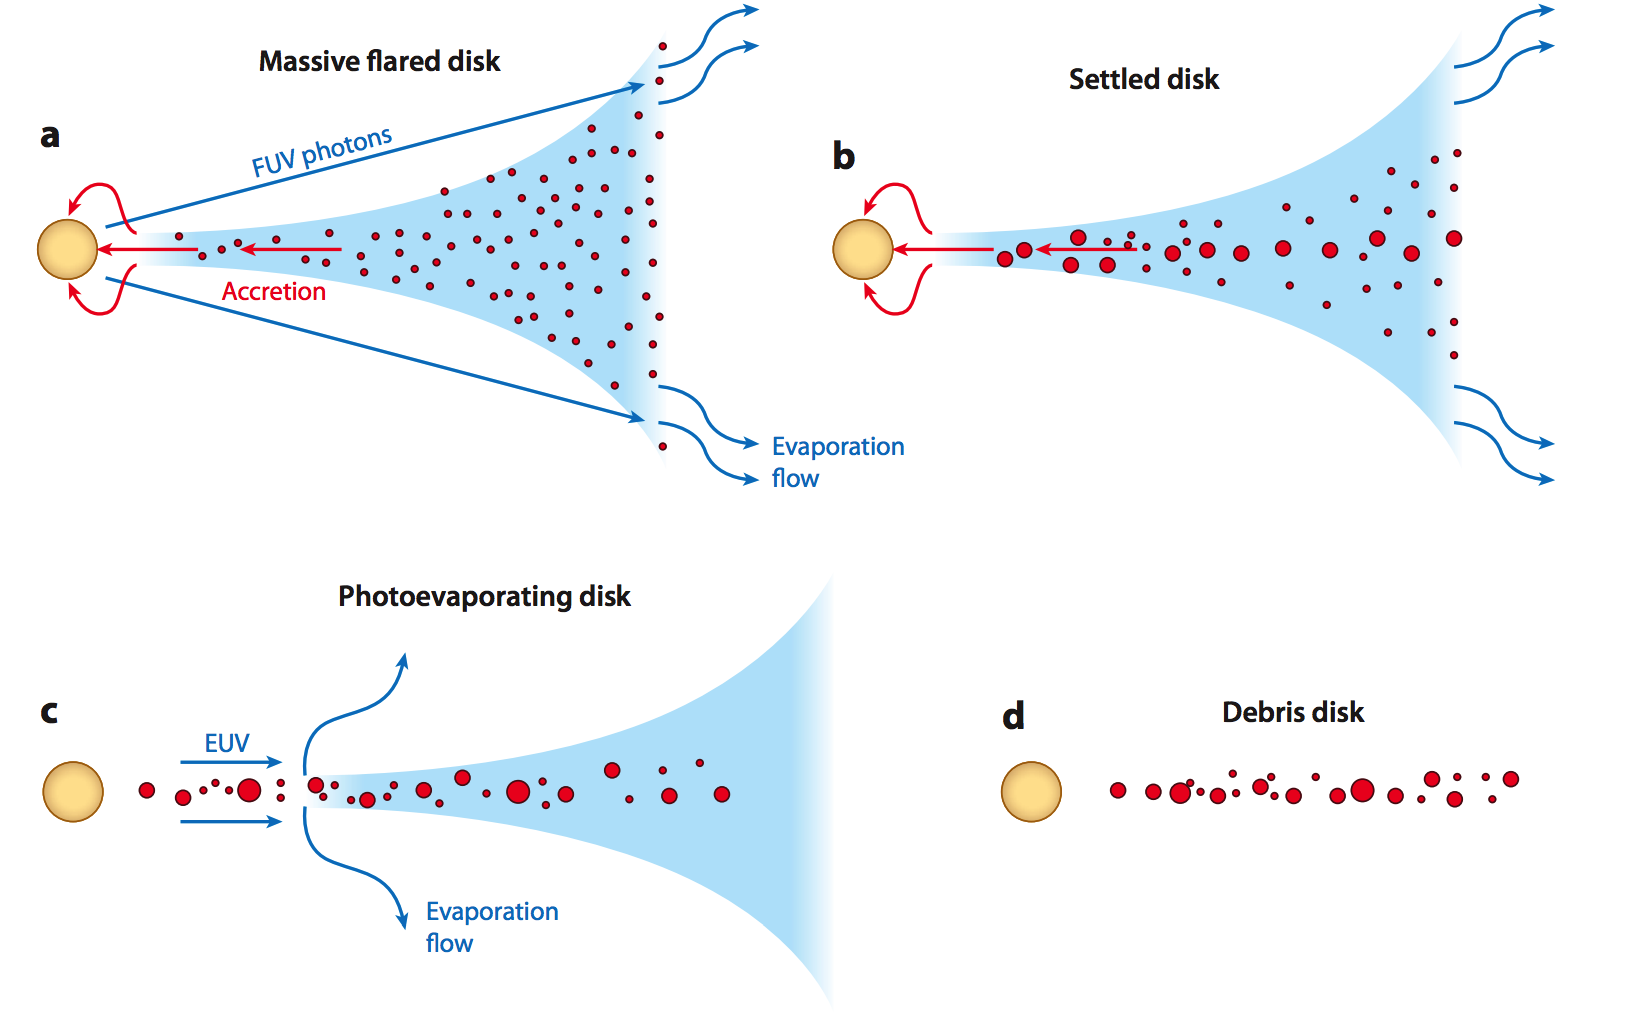
\includegraphics[width=\textwidth]{Ch1/disk_evolution_wc2011} 
    \caption[Disk Evolution Mechanisms]{Placeholder -- will use different figure of my own making. Right now from \citep{Williams2011}}
    \label{fig:ppd_2_dd}
    \end{figure}
    %===================================================================
    
    Observations have shown that once the inner disk ($<$5~AU) is depleted, the outer disk quickly loses the majority of its mass \citep{Williams2011}. Thus, after about 6--10 Myr, most stars have lost their inner disks, as determined from the stars near-IR excess emission \citep{Wyatt2008}. Figure~\ref{fig:ppd_near_irexcess} shows the rapid decline in disk fraction as a function of age for a number of different young stellar clusters and associations, illustrating that the fraction of stars with near-IR excesses dwindles down to $\sim$0\%. 
    
    %===================================================================
    %   EVOLUTION OF NEAR-IR EXCESS IN PPDS WYATT2008 FIG 2
    %===================================================================
    \begin{figure}
    \centering
    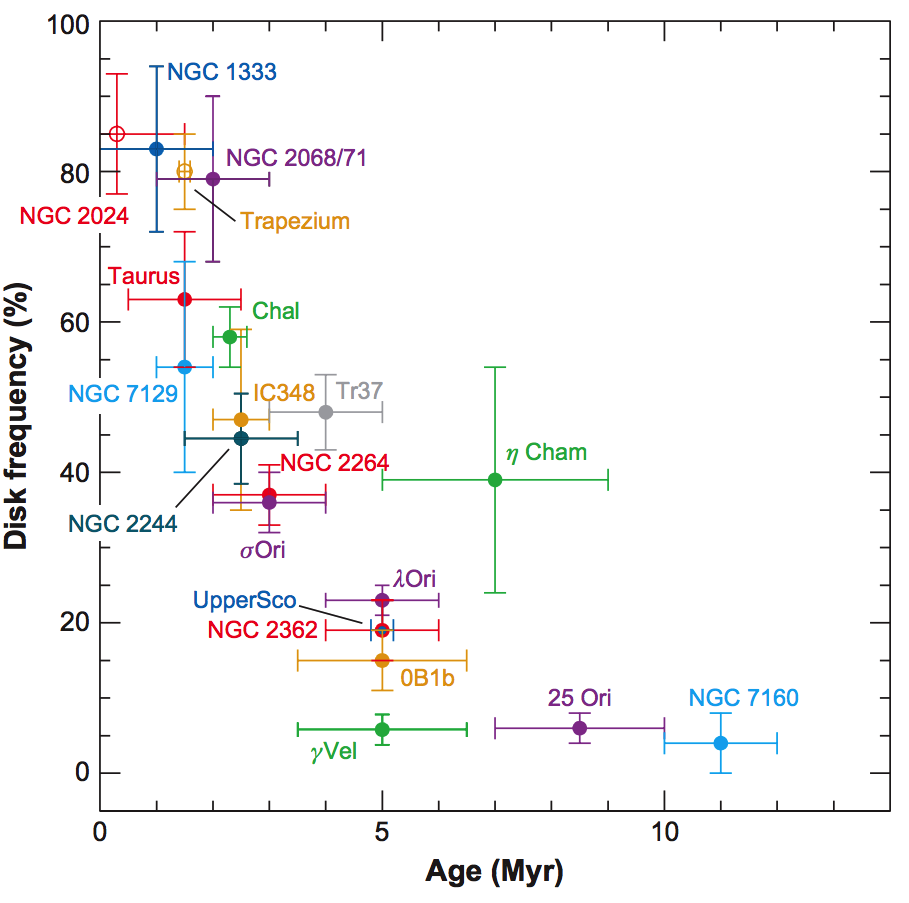
\includegraphics[width=\textwidth]{Ch1/diskfraction_vs_age_wyatt2008}
    \caption[Protoplanetary Disk Fraction Evolution]{Fraction of young stars in different associations, groups, with protoplanetary disks as detected via their near-IR excess flux. By around 6--10~Myr, the fraction of stars with a protoplanetary disk is almost zero. Figure taken from \citet{Wyatt2008}.}
    \label{fig:ppd_near_irexcess}
    \end{figure}
    %===================================================================
    
        
    \subsection{Debris Disk Evolution}\label{sec:debrisdisk_phase}
    
    \subsubsection{Dust Removal Mechanims}
    What remains from the remnant PPD after the bulk of the gas has dissipated, is typically a disk composed of planetesimals and dust population (illustrated in Figure~\ref{fig:ppd_2_dd}). From studies \citep[e.g.,][]{Lisse2009, Lisse2012, deVries2012, Rodigas2015} we know that the dust in a circumstellar disk can be composed of solid particles, ranging in sizes from mm to $<100$\micron\ in size and heterogeneously composed of various minerals: silicates, other dielectric and refractory particles, and ices (e.g., ice, Carbon Monoxide). We know from observations of debris disks at sub-mm wavelengths that dust masses are orders of magnitudes lower than in the gas-rich PPD phase; typically on the order of less than an Earth mass (see Figure~\ref{fig:disk_masses}). 

    The motions of grains larger than $\sim$1~mm (e.g., large grains, small planetesimals), are governed by the gravitational force from the central star. The low mass of these disks implies  debris disks are optically thin, meaning that the majority of the radiation that passes through the disk is seen by the observer. Hence thermal emission seen from these disks is typically due to smaller grains of order $s<1$~mm. For these smaller grains of size $s<1$~mm, stellar radiation and stellar wind play an important role in the dynamical behavior of the dust. The force exerted on a particle from radiation pressure $\vec{F}_r$ counteracts the radial gravitational force, giving rise to the photo-gravitational force
    
    \begin{equation}\label{eq:photograv_force}
    \left|\vec{F}_{pg}\right|= \frac{GM_\star m_d(1-\beta)}{r_d^2},
    \end{equation}
    
    \noindent where $\beta$ is the ratio of the radiation to gravitational pressure, and is inversely proportional to the stellar luminosity, grain density and size \citep{Burns1979}. In other words, smaller particles will be influenced largely by radiative forces, rather than gravitational ones. Grains whose bulk and optical properties produce $\beta=0.5$ experience equal gravitational and radiation pressure and represent the minimum size $s$ below which grains will be ejected from the system (blow-out size). In the Solar System, this corresponds to sub-micron sized grains. In addition to radiation pressure, stellar wind pressure created from high velocity plasma, aids in counteracting the gravitational force dust grains feel. 

    %===================================================================
    %   PR Drag
    %===================================================================
    \begin{figure}
    \centering
    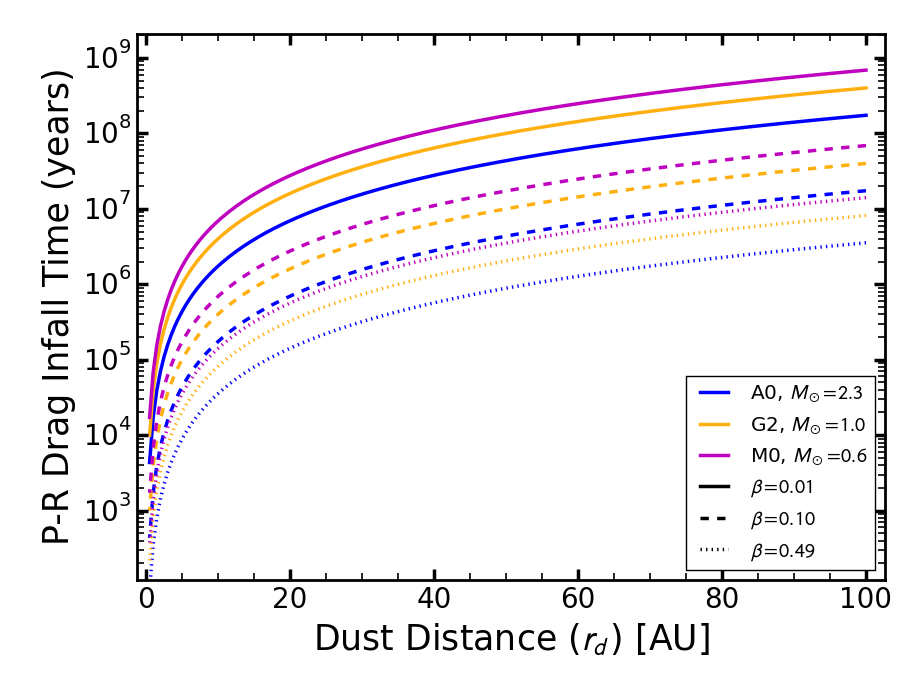
\includegraphics[width=\textwidth]{Ch1/PR_Drag_time} 
    \caption[Poynting-Robertson Drag Timescales]{A plot of the time it takes for dust at a distance $r_d$ to spiral into the star due to P-R drag. The model for these curves are based on the derivations of \citet{Burns1979}: $t_{pr}=400(r_d^2/M_\star)\beta^{-1}$. Large values of $\beta$ represent smaller particles, and vice-versa. I have plotted the curves for different values of $\beta$ and for different spectral types (stellar masses).}
    \label{fig:PR_Drag_time}
    \end{figure}
    %===================================================================
    
    Drag forces will cause the dust to slow down and spiral out of its orbit and eventually into the star. The tangential component (i.e., along the motion vector of the grain), of the stellar wind, or corpuscular drag, is one such drag force. This becomes more important for grains smaller than 0.001\micron\ around Sun-like stars\citep{Burns1979}. The tangential component of the stellar radiation also creates a drag-force on the particle known as Poynting-Robertson (P-R) drag. P-R drag relies on the change in a particle's momentum due to the acceleration it feels from the stellar radiation perpendicular to its motion vector, and the deceleration it feels from re-radiating the absorbed stellar radiation along the particle's velocity vector. 
    
    
    \begin{equation}\label{eq:pr_drag}
    |\vec{F}_{PR}| = \frac{S\pi a^2 Q_{PR}r_d^2 v}{c^2},
    \end{equation}
    
    \noindent where $S$ is the stellar flux density, $Q_{PR}$ is the radiation pressure coefficient, and $v$ is the velocity of the grain in the direction normal to the radiation vector \citep[i.e., orbital direction;][]{Burns1979}. 
    
    \textbf{P-R drag works by an inhomogeneous momentum exchange...reword}.
    
    Figure~\ref{fig:PR_Drag_time} shows that dust around most main-sequence stars at $r_d<15$~AU will spiral into the star on timescales $\lesssim 100$~Myr. It will take longer for grains at larger distances to spiral into the star, in which case radiation pressure and stellar wind will throw grains out of the system. However, in most detected debris disks (discussed in \S~\ref{sec:thirty_years}), collisions grind down grains on shorter timescales than P-R drag can remove them from the system \citep[e.g.,][]{Wyatt2008}. Grains, once ground down to smaller sizes can then be removed from the system more easily by radiation pressure and stellar winds. For instance, 100\micron\  grains at 90~AU from the star Vega will spiral into the star within 15~Myr. With collisions, these grains will be removed in roughly 2~Myr \citep{Backman1993}. 
    
    \subsubsection{Dust Replenishment And Planetary Stirring}\label{sec:replenishment}
    
    We now know that any initial population of dust in a circumstellar environment will not last the lifetime of the star. The larger main-sequence stars, of spectral type (SpT) A2V and earlier, live for $<$500~Myr. Dust, on the other hand, is only stable around a star for timescales $\lesssim 1-10$~Myr (dependent on the luminosity of the star in question; see Figure~\ref{fig:PR_Drag_time}). 
    
    Over the last thirty years, over a thousand debris disks have been discovered. In light of the theory in the preceding sections, what would be surprising to the uninitiated is that these debris disk systems have been detected around stars of all main-sequence spectral types, as well as ages well beyond the timescale of dust dissipation Figure~\textbf{Figure of dust brightness vs. age}. 
    
    %===================================================================
    %  DUST BRIGHTNESS VS AGE PLOT
    %===================================================================
    %\begin{figure}
    %\centering
    %\includegraphics[width=\textwidth]{Ch1/??} 
    %\caption[??]{??}
    %\label{fig:??}
    %\end{figure}
    %===================================================================
    
    A well accepted explanation for the existence of dust around main-sequence stars is that the dust is replenished from the destructive collisions of larger oligarchs, planetesimals, asteroids, comets, etc, where a lot of the dust mass is locked up. The collisions may occur through steady state evolution, whereby larger bodies and grains are ground into smaller sizes, eventually being thrown out of the system through one of the dissipative forces described earlier. Thus, a collisional cascade ensures, creating a size distribution of particles. Smaller particles will be removed from the system quickly, while larger particles replenish the smaller grain population. This cycle removes mass from the disk on timescales $\propto t^{-1}$ \citep{Wyatt2007}. Stochastic evolution may also be responsible for dust replenishment, where dust is ejected into the system from sudden collisions. The LHB event in the early Solar System is an example of this type of dust generation. 
    
    For collisions to occur, grains and planetesimals must have enough kinetic energy. It is possible that disks evolving from the PPD phase are self-stirred to generate a collisional cascade. Delayed and self-stirring models, whereby the planetesimal disk is stirred from the influence of larger bodies once they have grown to sizes $>$2000~km, have also been successfully been used to explain the presence of dust. As stated by \citet{Wyatt2008}, for continuous belts between 1--200~AU, differences between self- and pre-stirred models are insignificant, but are most apparent when there is a clearing in the inner regions.
    
    Though there are a number of collisional models which can adequately explain the dust production in observed systems, the details of each model are beyond the scope of this dissertation. Suffice it to say that the presence of circumstellar dust around main-sequence stars is due to the collisional cascade of planetesimals that ensues from dynamical perturbations.
    
\section{Detecting Debris Disks}\label{sec:detect_dd}

    \subsection{Dust Thermal Emission}

    Circumstellar dust immersed in the radiation field of its host star will both scatter and absorb incoming radiation. Though most types of grains are efficient scatterers in the optical and near-IR (see \S~\ref{sec:excess_resolvedimaging}), a fraction of that light is absorbed and heats the dust. Smaller grains will heat up faster and hence radiate more efficiently than larger grains of the same composition and at the same distance \citep{Krivov2010}. However, differentiating scattered versus stellar radiation becomes difficult since main-sequence stars at $T_\star>3000$~K have peak emission in the optical and near-IR (0.4--2.5\micron), thus decreasing the contrast between scattered and stellar light in these regimes. Reprocessed thermal emission is easier to detect, as emission from the dust peaks in the mid (10--30\micron) and far-IR ($>30\mu m$) wavelengths --- regimes where the stellar photospheric emission can be order of magnitudes fainter than the observed thermal emission.  
        
    %===================================================================
    %   IR Excess Illustration
    %===================================================================
    \begin{figure}
    \centering
    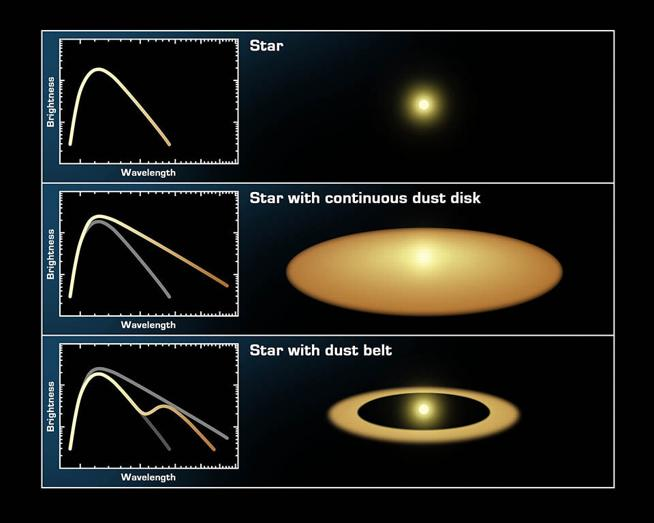
\includegraphics[width=\textwidth]{Ch1/IR_Excess_diagram} 
    \caption[]{}
    \label{fig:PR_Drag_time}
    \end{figure}
    %===================================================================

    Small dust grains, on the order of tens of microns, are largely responsible for thermal emission seen from a star in the mid- and far-IR, given their efficient emission properties. It is typically assumed that the grains are in thermal equilibrium with the stellar radiation field. The amount of energy a grain absorbs (mainly in the UV and optical) $E_{abs}$, is dependent on its size $a$, radial distance from the star $r_d$, stellar luminosity $L_\star$ and the absorption efficiency $Q_{abs}(a,\lambda)$
    
    \begin{eqnarray}\label{eq:energy_absorbed}
    E_{abs} &=& \left(\frac{\pi a^2}{4\pi r_d^2}\right) \int_0^\infty L_{\lambda} Q_{abs}(a,\lambda) d\lambda \\
            &=&  \frac{a^2}{4r_d^2}L_\star \langle Q_{abs}\rangle_{UV}. 
    \end{eqnarray}
    
    \noindent The energy emitted by the grain $E_{r}$ depends on the grain size, the radiative efficiency $Q_{r}(a,\lambda)$, and is approximated by
    
    \begin{eqnarray}
    E_{r} &=& 4\pi a^2 \int_0^\infty \pi Q_{r}(a,\lambda) B(\lambda,T_d)  d\lambda \label{eq:energy_emitted1}\\
          & \approx & \left(2\pi a\right)^2 \sigma T_d^4 \langle Q_{r}\rangle_{IR}. \label{eq:energy_emitted2}
    \end{eqnarray}
            
    
    \noindent As standard practice, I've assumed an average absorption and emitting efficiency for the grain, which can be derived using Mie Theory. If we assume the grain emits as a blackbody, the expression derived in equation~\ref{eq:energy_emitted2} naturally falls into place. Conservation of energy dictates that
            
            
    \begin{equation}\label{eq:conserve_energy} 
     \frac{a^2}{4r_d^2}L_\star \langle Q_{abs}\rangle_{UV} \approx \left(2\pi a\right)^2 \sigma T_d^4 \langle Q_{r}\rangle_{IR},
    \end{equation}
            
    \noindent which leads to an approximate expression to calculate the dust temperature
    
    \begin{equation}\label{eq:tdust_full}
    T_d \approx \left(\frac{\langle Q_{abs} \rangle_{UV}}{\langle Q_{r}\rangle_{IR}} \frac{L_\star}{16\sigma \pi^2 r_d^2}\right)^{1/4}.
    \end{equation}
        
    In most cases, the amount of information obtained from the dust emission is only sufficient to satisfy the simplest emission models: grains that emit as blackbodies. In the blackbody assumption, equation~\ref{eq:tdust_full} reduces to 
            
    \begin{equation}\label{eq:blackbody_temp}
            T_d = 278 \frac{\left(L_\star/L_\odot \right)^{1/4}}{\sqrt{r_D}}\enspace [K]. 
    \end{equation}
    
    \noindent assuming that $\langle Q_{abs} \rangle_{UV} \approx \langle Q_{r}\rangle_{IR}$. In a more general sense, the grain equilibrium temperature can vary as it depends on the composition and size of the grain\citep{Draine2003}. Grains that deviate from the blackbody approximation will have non-zero absorption and emission efficiencies, and moderate the slope of the Wien and Rayleigh-Jeans tails of the grain emission spectrum. Around a Sun-like star, unless the dust orbits at $r_d<0.1$~AU, the grain temperatures will typically be $T_d \lesssim 300$~K. Following Wien's approximation, this means that the dust emission spectrum will peak in the mid- and far-IR wavelengths. Thus, astronomers will usually search for the presence of dust at IR wavelengths. 

    \subsection{Infrared Excess and Resolved Imaging}\label{sec:excess_resolvedimaging}

    In 1983, the Infrared Astronomical Satellite (\iras) was launched through a joint initiative between NASA in the United States, the Netherlands Agency for Aerospace Programmes and the Science and Engineering Research Council in the United Kingdom. By the end of its 10 month mission, \iras\ had mapped 96\% of the sky at 12, 25, 60 and 100\micron. This was the first time the entire sky had been imaged in the IR. 
    
    %===================================================================
    %   First IR Excess From \iras\
    %===================================================================
    \begin{figure}
    \centering
    \begin{tabular}{c}
    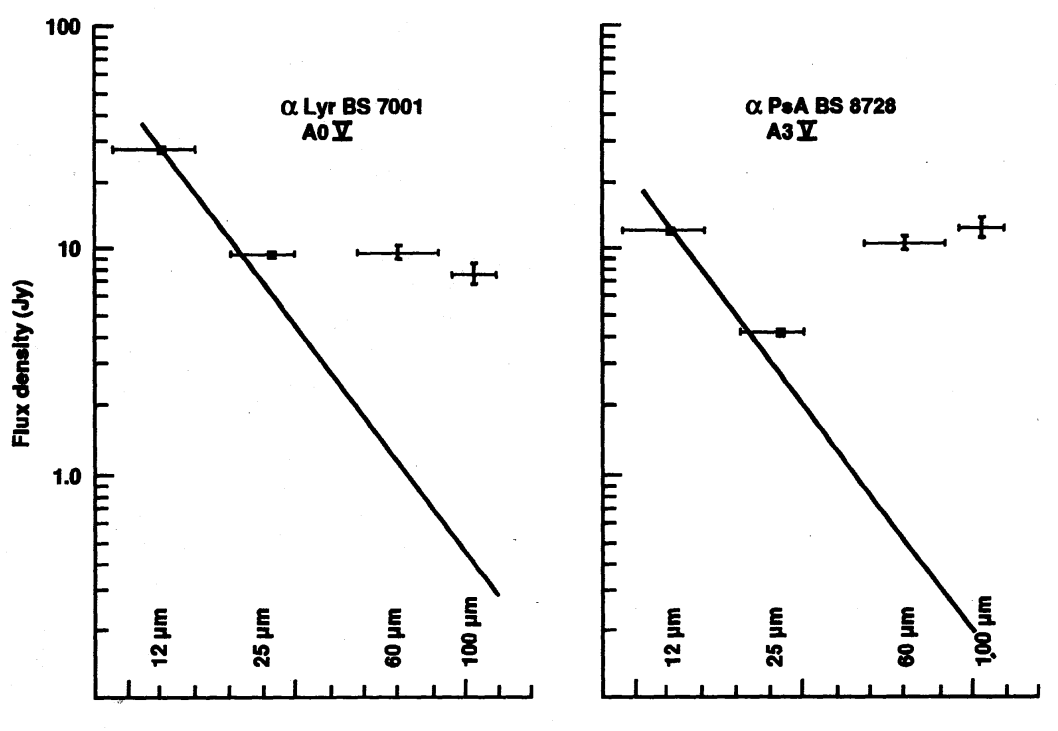
\includegraphics[width=.7\textwidth]{Ch1/backman_parsece_1993_IRExcesses_1}  \\
     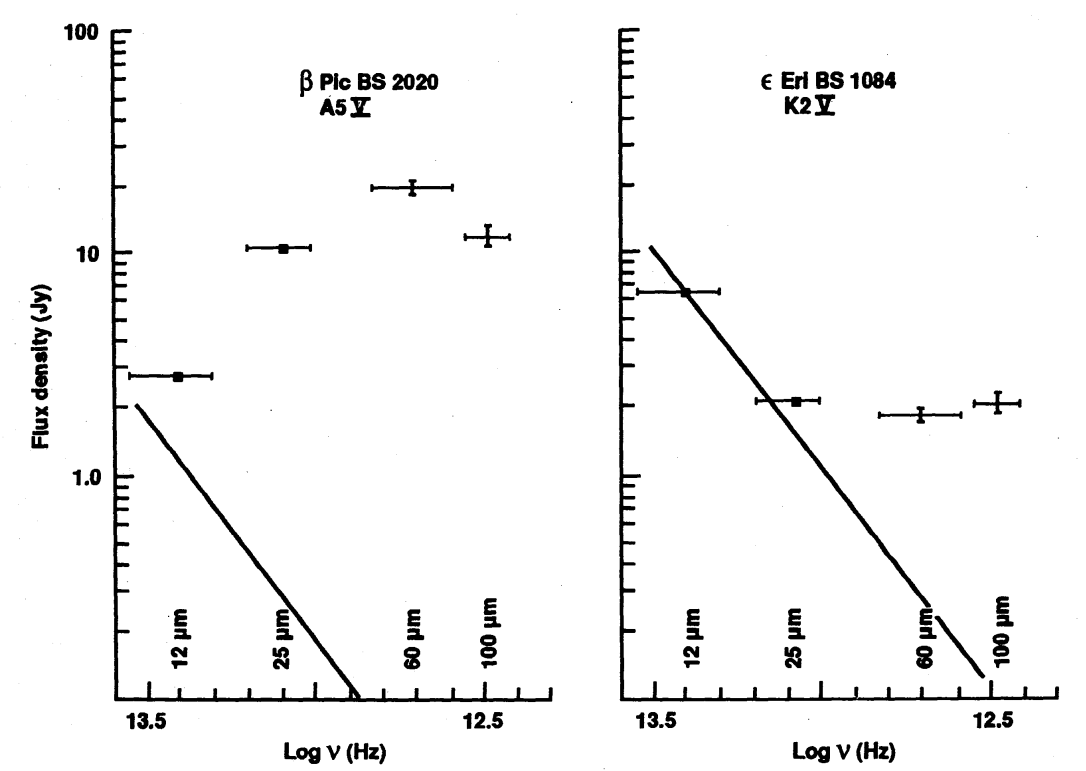
\includegraphics[width=.7\textwidth]{Ch1/backman_parsece_1993_IRExcesses_2}
    \end{tabular}
    \caption[SEDs of Fab Four Disks]{The SEDs of four stars taken from \citet{Backman1993}. Starting from top-left and moving clockwise: Vega ($\alpha$~Lyr), Fomalhaut ($\alpha$~PsA), $\epsilon$~Eridani, and $\beta$~Pictoris. The \iras\ fluxes of these stars are shown at 12, 25, 60 and 100\micron\ with the Rayleigh-Jeans photospheric flux over-plotted. The large excess flux measured for these stars indicates optically thin circumstellar disks of cold micron sized grains. These were the first four disks discovered around main-sequence stars, hence named \textit{The Fab Four}.}
    \label{fig:fab_four}
    \end{figure}
    %===================================================================
    
    
    
    Measurements of a few standard stars revealed a peculiar behavior: where they expected a Rayleigh-Jeans trend in the flux as a function of wavelength, they found instead that the measured fluxes of several stars like Vega ($\alpha$ Lyr), Fomalhaut (HD~216956), $\beta$~Pic (HD~39060), and $\epsilon$~Eridani revealed an excess of flux several orders of magnitude above the predicted photospheric flux at two or more of the longer wavelength bands. This has since been attributed to ``a shell or ring of relatively large particles'' at distances and that the grain equilibrium temperatures are $\sim90$~K \citep{Aumann1984, Backman1993}. Figure~\ref{fig:fab_four} shows the theoretical spectral energy distributions (SED) of these four stars in the Rayleigh-Jeans regime, along with the measured fluxes from \iras.
    

    The majority of disk systems are identified through unresolved emission via photometric or spectroscopic imaging techniques. The IR emission from a star with dust is compared of both the stellar and dust flux. To characterize the dust emission, astronomers must accurately measure and subtract the flux from the star. Fits to stellar models use photometric or spectroscopic data collected in the optical and near-IR ($0.9-5$\micron), where the luminosity of the star is large enough to overwhelm the thermal emission from dust at temperatures $<300$~K. The fitted photospheric emission is then extrapolated to the IR. Figure \textbf{SED figure with model fit} shows this fit along with the blah blha blah. Thus, the excess flux at a particular wavelength is a simple subtraction
    
    \begin{equation}\label{eq:excess+flux}
    F_{E,\lambda} = F_{m,\lambda} - F_{\star,\lambda},
    \end{equation}
    
    \noindent where $F_{m,\lambda}$ and $F_{\star,\lambda}$ are the measured and photospheric fluxes, respectively. The amount of excess flux at a particular wavelength can be characterized by the measured flux to the photospheric emission, or the relative flux of the excess
        
        \begin{equation}\label{eq:rel_excess}
        R_\lambda = F_\lambda / F_{\star,\lambda}.
        \end{equation}
        
        \noindent The fractional luminosity of the IR excess $f_d$ characterizes the total emission spectrum, or bolometric luminosity, of the dust with respect to the bolometric stellar luminosity
        
        \begin{equation}\label{eq:fd}
        f_d = L_{IR}/L_{\star}.
        \end{equation}
        
        \noindent The fractional luminosity can provide a rough estimate of the mass of the dust in the system. This calculation is proportional to $f_d$ as well as the bulk density, grain size, and location from the star \citep{Beckwith2000}. 
        
        However, attributing IR excesses based on unresolved fluxes to be circumstellar in nature is not an easy task. There are numerous astrophysical and systematic sources that can contaminate or mimic an IR excess. Background extra-galactic sources (e.g., active galactic nuclei, IR bright galaxies), unresolved projected stellar companions and thin patches of infrared bright clouds of dust are only a few sources that can mimic and bias the detection of an IR excess. Screening of potential contaminants must be done with great care; follow up studies of potential disk systems are also required to verify the observed thermal excess emission is associated with circumstellar dust.
        
    Resolved images of a debris disk can verify and validate the circumstellar presence of an excess by revealing the structure of the disk. Most resolved disks\footnote{See \url{http://www.circumstellardisks.org} for a compilation of resolved disks.} have been imaged in the optical to near-IR wavelengths. Since the star is orders of magnitudes brighter than the scattered emission from the dust in these wavelength regimes, high-contrast imaging techniques must be employed. This usually done by using an opaque disk, known as a coronagraph, to attenuate/block the on-axis stellar light. Coronagraphic techniques reduce the glare from the star and allow faint, nearby structure to be imaged. The first resolved image of $\beta$~Pic (Figure~\ref{fig:smith_terrile_betapic}) was taken using a coronagraph and imaged in the optical at the Las Campanas Observatory.
        
    Current high-contrast imaging instruments at most ground based observatories also require an adaptive optics (AO) instrument to correct for the refractive distortions imprinted on the stellar wavefront as it passes through our turbulent atmosphere. New extreme-AO systems \citep[e.g., Gemini Planet Imager,][]{Macintosh2006} are well equipped to image separations as close as 10~AU to some of the closest stars. Information from resolved disks are important as they elucidate degenerate disk parameters obtained from simply analyzing unresolved dust emission. For instance, modelling the SED of the IR excess can be done by either assuming small grains further from the star, or large grains close to the star \citep{Krivov2010}. Thus, the location of the dust that is causing the emission is important to break the degeneracy\citep[e.g., Figure 13][]{Su2006}. 
        
        
    \subsection{Is It A Protoplanetary Or A Debris Disk?}
    
    As illustrated in Figure~\ref{fig:ppd_2_dd}, the transition out of a PPD, broadly speaking, occurs with the dissipation of the primordial gas. The remnant circumstellar environment can be composed of planets, minor bodies (asteroids and comets), and micron to mm sized dust grains, which may have formed during the PPD phase. This post-PPD, gas depleted, dust-rich disk is known as a ``Debris Disk.'' %For the next two sections, I will elucidate the characteristics and dynamics that govern this post-PPD debris-rich phase.
    
    However, there is no clear dividing line between the waning of a PPD and the waxing of a debris disk. Age is one dividing line, though there are examples of PPDs that are older than 30~Myr \citep{DeMarchi2013,Scicluna2014}, and debris disks that have been found in young clusters. The mass of the disk can also be an indicator, as PPDs are usually a couple of orders of magnitudes more massive than in a debris disk, as shown in Figure~\ref{fig:disk_masses}. A debris disk, unlike a primordial disk, has a smaller gas to dust ratio. Since these disks are primarily optically thin, their IR excesses, and consequently their fractional luminosities, are smaller. Therefore, a debris disk can be characterized by $f_d<10^{-2}$ \citep{Zuckerman2001, Wyatt2008}. 
    
    Although there are clear physical traits that debris disks possess, it is important to note that there can be ambiguities in the disk status of a certain system. Guidelines, like those listed in \citet{Wyatt2015}, can aid in clearing such distinctions. However such effort will not be placed here as it is beyond the scope of this thesis.
    
    
\section{Debris Disk as Signposts for Planets} \label{sec:disks_signposts_planets}
    
    The self-stirred models, which I briefly touched upon in \S~\ref{sec:replenishment}, have vast implications for concurrent belt and planetary evolution. Although other mechanisms, such as pre-stirring or close-stellar encounters are possible for generating the necessary perturbations to start a collisional cascade, there is evidence, both theoretical and observational, of dust generation due to the influence of planets \citep[e.g., the HD~141569 system,][]{Wyatt2005}. Plus, with the large number of exoplanets discovered every year, and statistical inferences that almost every star is host to a planetary system \citep{Cassan2012}, dust generation via planetary perturbations is likely a significant phenomenon. At the same time, this presents us with an opportunity: if dust in debris disks is generated from collisions due to the influence of larger planetary objects, then the \textit{dust may act as a signpost for undiscovered planetary systems}.
    
    Unresolved debris disk detection can reveal much about the activity in a planetary system. Any excess flux attributed to the star can be used to roughly determine the amount of dust in that system. For stars that are a few hundred million years old, large excess fluxes imply recent collisions, as primordial dust from young systems would have been dissipated millions of years prior \citep[e.g., BD+20 307;][]{Song2005}. In addition, a number of studies have attempted to determine the correlation between systems with known disks and detected planets. The likelihood of a disk being found with known directly imaged systems is relatively high (e.g., systems like $\beta$~Pic and HR~8799), studies that have tried to find correlations between planet hosts and disk hosts have found conflicting results with strong to no correlation between the two \citep[mainly seen with Spitzer studies;][]{Beichman2005, Bryden2009}. More recent studies with \textit{Herschel} seem to provide more evidence of a positive correlation between cold disks with the presence of low mass planets \citep[see references in][]{Matthews2014}. In essence, a broader characterization of dust around known planet hosts, or vice versa, is necessary to discern the true correlation of this relationship.

    Resolved images can reveal structure in the observed debris disk such as gaps, warps, brightness peaks, etc., which can clarify the dust composition, as well as act as fingerprints for possible planetary activity. For instance the shape of the disk in scattered light can be used to place upper limits on the mass of giant planets sculpting the disk \citep[e.g.,][]{Kalas2005b,Rodigas2014}. The warp and secondary dust ring seen in scattered light in the $\beta$~Pic system was evidence for a possible planet sculpting the ring, as seen in Figure~\ref{fig:betapic_diskplanet} \citep{Heap2000}. Later observations in 2010 confirmed the existence of a $9\pm2.5 M_J$ planet via direct imaging \citep{Lagrange2010, Marleau2014}. The recent CO gas clumps seen in this system by the Atacama Large Millimeter/submillimeter Array (ALMA)\footnote{\url{http://www.almaobservatory.org/}} in Chile are thought to be the result of spiral density waves of dust, created in from the gravitational influence of $\beta$~Pic~b \citep{Nesvold2015}. 

    %===================================================================
    %   Resolved Disk Imaging - Beta Pic
    %===================================================================
    \begin{figure}
    \centering
    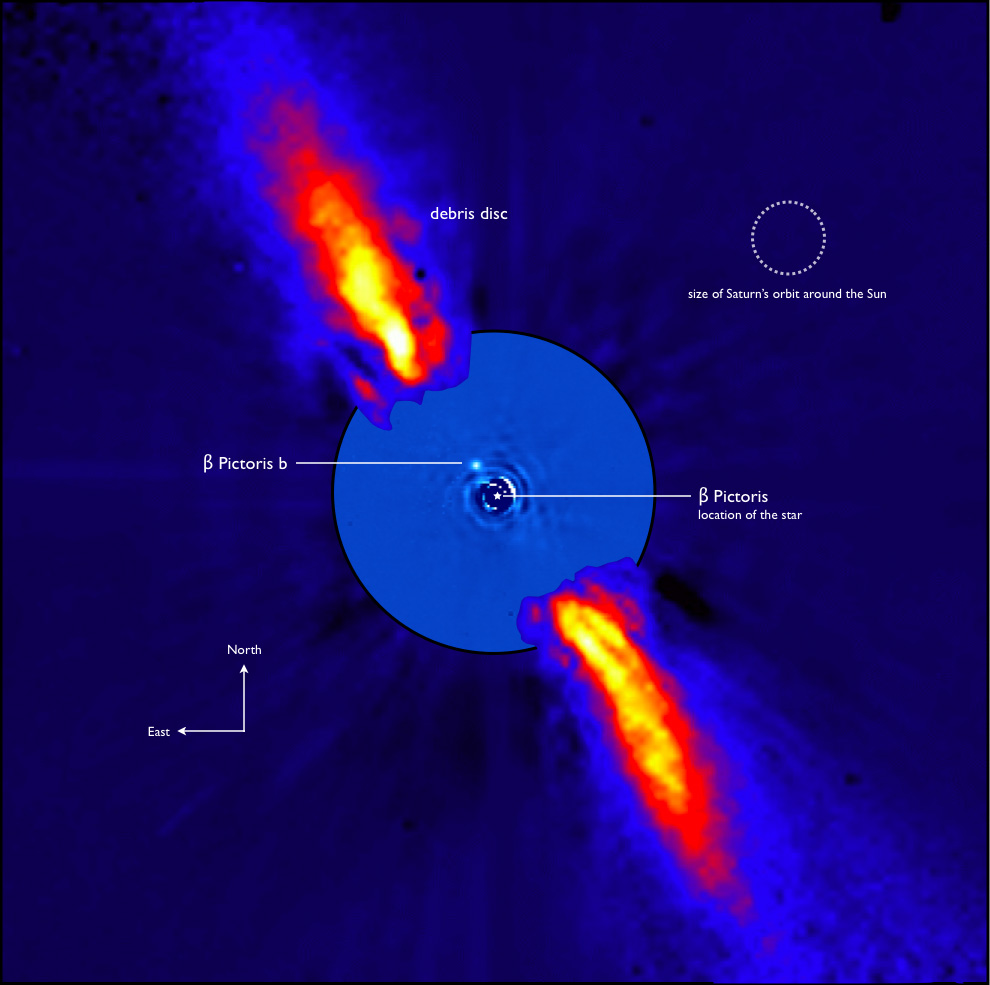
\includegraphics[width=0.7\textwidth]{Ch1/Beta_Pictoris_planetdisk}
    \caption[$\beta$~Pictoris Disk and Planet]{A composite image of the $\beta$~Pic debris disk over plotted with the discovery image of the gas giant planet $\beta$~Pic~b \citep{Lagrange2010}. The warp and secondary inclined disk were evidence of the infludence of the planet found in 2008 and later confirmed in 2010.}
    \label{fig:betapic_diskplanet}
    \end{figure}
    %==================
    
    
    
    %===================================================================
    %   Resolved Disk Imaging - Liou & Zook
    %===================================================================
    \begin{figure}
    \centering
    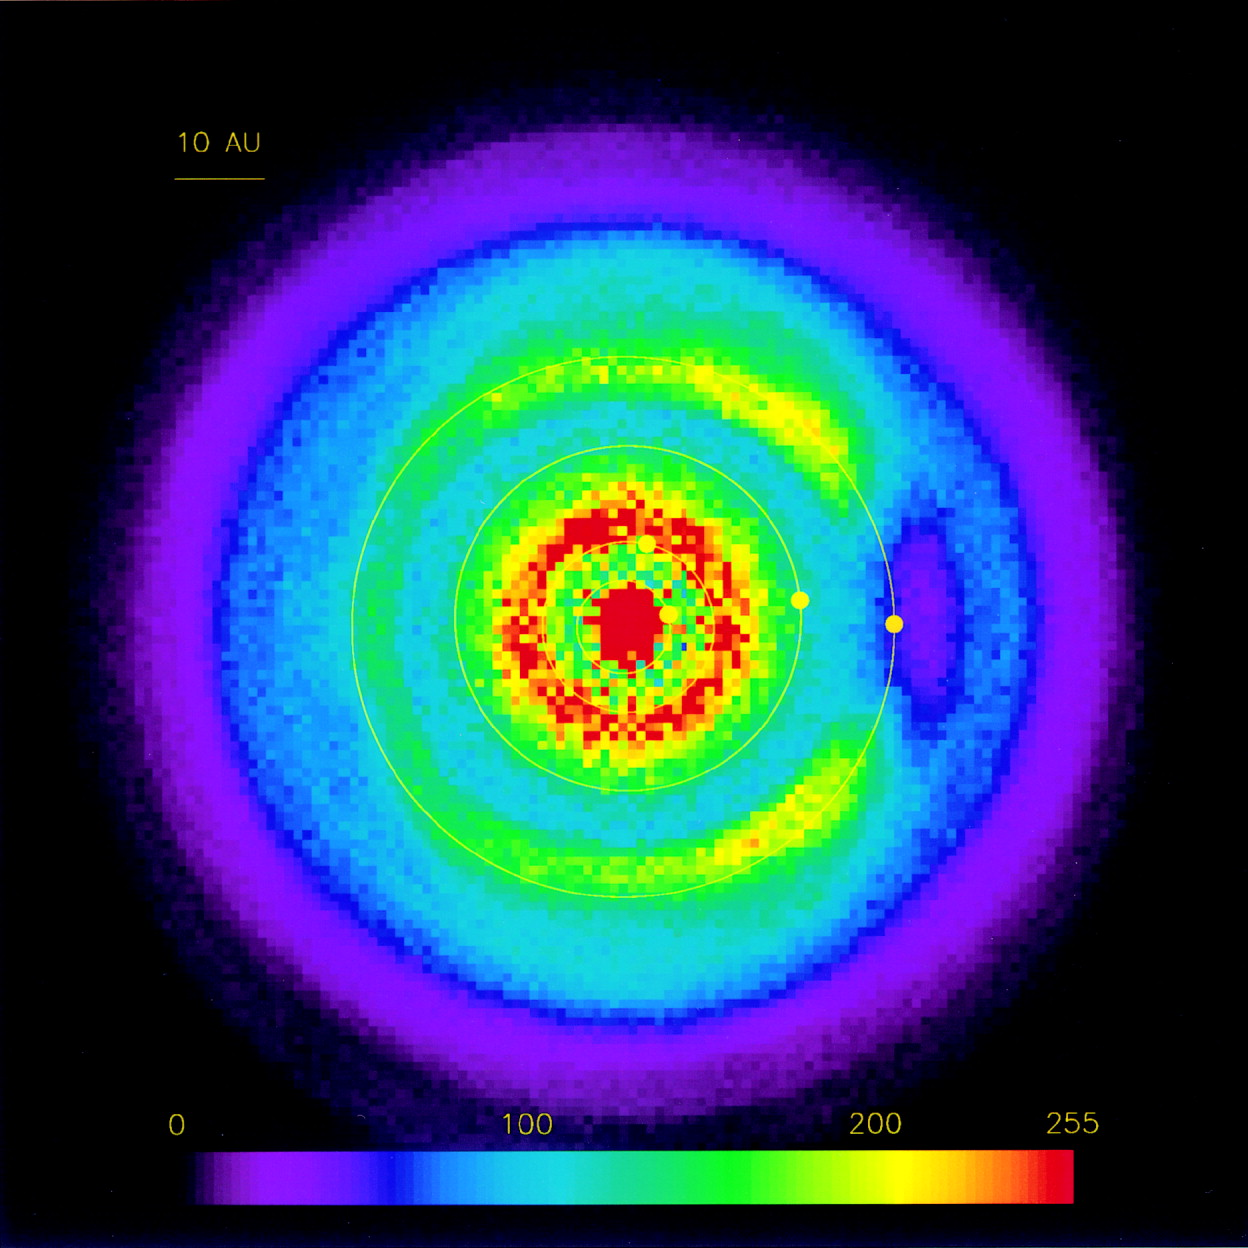
\includegraphics[width=\textwidth]{Ch1/LiouZook_SS_99}
    \caption[Giant planets imprinted on solar system disk simulation]{Simulation of the brightness distribution due to 23\micron\ interplanetary dust in a face-on view of the solar system made by \citet{Liou1999}. Shown are the four giant planets in the Solar System, with Neptune's orbit and gravitational influencing the outer architecture of the EKB, and Jupiter and Saturn ejecting particles that are gravitating inwards. From this image, the existence of at least 2 planets can be discerned.}
    \label{fig:LiouZook_faceon}
    \end{figure}
    %==================


    Using multi-wavelength modeling of resolved images from the Herschel Space Telescope of the Fomalhaut debris disk system, \citet{Acke2012} showed that cometary collisions were responsible for the dust seen in the disk. The planet in the Fomalhaut system \citep{Kalas2008} was discovered from direct imaging observations after the dust ring in the system was thought to have been sculpted by the Fomalhaut~b planet. Although the detected planet is not responsible for the current architecture of the ring \citep{Kalas2013}, it leaves the door open to additional discoveries. And recently, \citet{Rodigas2014} derived an analytical expression to determine the mass of a planet interior to any debris ring scattered light observations. 
    
    As discussed in \S~\ref{sec:solar_system}, the architecture of the circumsolar debris disk also contains clues on the influence the planets have had. Gaps in the Asteroid belt, known as the Kirkwood gaps, are the result of the unstable resonant structures due to Jupiter's orbit. Both the Asteroid belt and EKB are due to the influence of Jupiter and Neptune, respectively, and also responsible for the interplanetary dust \citep[e.g.,][]{Morbidelli2010}. An alien observer looking at our dust disk would be able to see gaps, non-uniform density distributions of dust and might infer the presence of at least three of the giant planets in the Solar System, as shown in Figure~\ref{fig:LiouZook_faceon} \citep{Liou1999}. What is clear at this point though is that the presence of dust around a star most likely indicates the existence of a complex planetary system, with complex architecture that has yet to be uncovered, or something as simple as illustrated in Figure~\ref{fig:planet_sandwich} --- planets sandwiched between dust belts --- like we see in our own Solar System.  
    
    
\section{Evolving Picture of Debris Disks Over Thirty Years}\label{sec:thirty_years}
       
    The majority of debris disks are discovered from the IR excess flux from the star, as opposed to resolved imaging which is typically done as followup to further characterize the disk properties. A number of different surveys have been responsible for the plethora of debris disks discovered to date. Here, I will give a brief summary of what we have learned from over last thirty years of disk detections, focusing largely on detections from unresolved IR excesses, statistics from various surveys as well as the evolutionary context they provide. The focus will be on detections from space based surveys such as \iras\, the \textit{Spitzer Space Telescope}, and \textit{Herschel Space Observatory}. Beyond what I discuss here, excellent reviews can be found in \citet{Zuckerman2001, Wyatt2008, Matthews2014}.  In addition, it is useful to keep in mind the relationship between the wavelength of detected dust emission to where the dust may be located as well as its temperature to first order. Figure~\ref{fig:planet_sandwich} provides a cartoon picture of these relationships. 
   
   %===================================================================
    %   MODEL EXOSOLAR SYSTEMS
    %===================================================================
    \begin{figure}
    \centering
    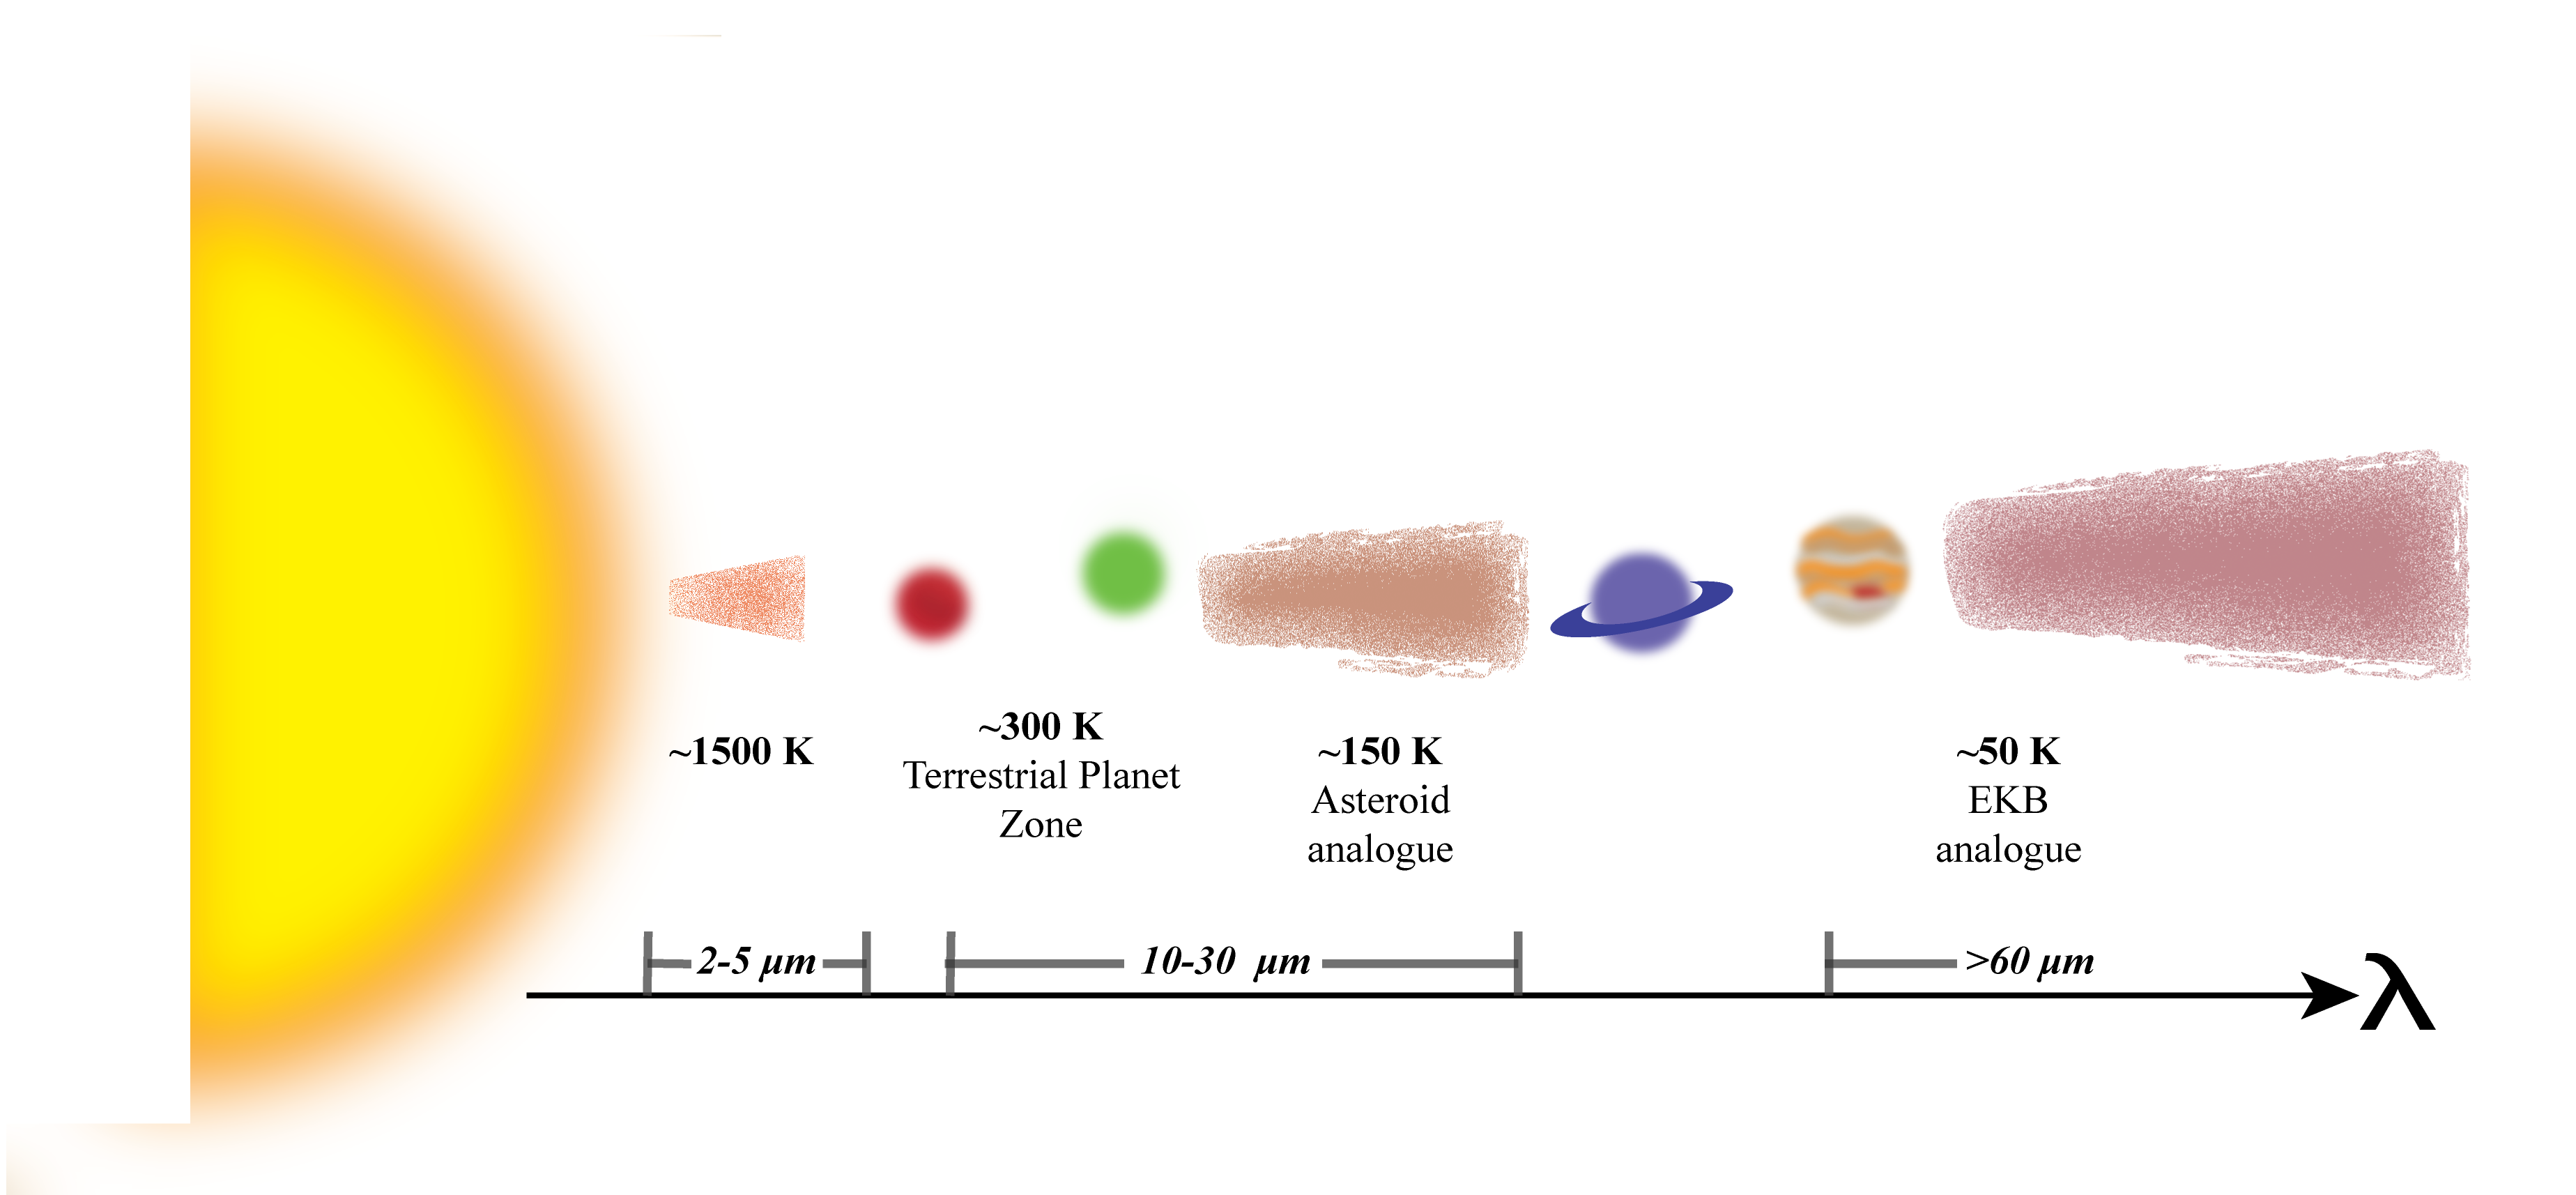
\includegraphics[width=\textwidth]{Ch1/planet_sandwich_RPatel}
    \caption[]{}
    \label{fig:planet_sandwich}
    \end{figure}
    %===================================================================
    
    
   
   
   Put different space emission paramters in appendix.
   
   - add in table of telescope sizes
   - add in table of instrument wavelength, sensitivity and resolution
   - add plot of sensitivity curves.
   
   
   
   \subsection{Cold Disk Detections}
   
   
    The few hundred debris disks originally detected by \iras\ via their far-IR (60--160\micron) excesses showed that these systems possess circumstellar dust in optically thin disks at relatively cold temperatures ($\sim$20--100~K). These temperatures, are derived from blackbody fits to the SED of the excess. The dust in these systems is analogous to dust in the EKB ($T_d\sim50$~K). Hence, the cold dust in these systems are signposts for dynamical planetary activity in the outer regions of these systems, in much the same way ethe cold dust in our system betrays the existence of Neptune, as it sculpts the cold planetesimal population in the EKB. 
   
   As mentioned previously, the early \iras\ detections mostly found dust around hotter A and B type stars and that roughly 15\% of these main-sequence stars are host to cold dust populations, detected at the \iras\ 60\micron\ band. Later studies that used improved versions of the original \iras\ database (Faint Source Catalog), identified a handful of new debris disk host stars, and increased the incidence of cold dust detections to 20\% \citep{Rhee2007}. The launch of the Spitzer Space Telescope in 2003 commenced a series of surveys to understand the evolution and existence of dust around nearby stars. The Formation and Evolution of Planetary Systems\footnote{\url{http://feps.as.arizona.edu/science.html}} \citep[FEPS;][]{Meyer2006} surveyed $\sim$300 stars between late A to late K spectral types at ages from 3~Myr to 3~Gyr. These studies found that cold dust, or excesses at the Spitzer/MIPS 70\micron\ band, was present around 33\% of A stars at all ages, and at relatively bright dust brightnesses \citep{Su2006}. The DEBRIS collaboration\footnote{Disc Emission via a Bias-free Reconnaissance in the Infrared/Submillimetre} recently published their results after conducting a survey for cold dust around 86 main-sequence A stars using the Herschel Space Observatory. They found that roughly 25\%$\pm$5\% of A stars possess far-IR excess emission at 100\micron \citep{Thureau2014}. 
   
   
   A similar search for cold dust around solar-type stars (F,G, and K spectra type) revealed something different. The incidence of excesses in the far-IR are lower and a stronger function of the age of the star than for the incidence of excesses around A stars. A number of Spitzer/MIPS 70\micron\ surveys \citep[e.g.,][]{Trilling2008, Bryden2006, Beichman2006, Hillenbrand2008} have found that on average, the incidence of 70\micron\ excesses is $\sim$ 15\%. \citet{Trilling2008} found $\sim16$\% of older stars in the field possess a far-IR excess, while these numbers are somewhat lower ($\sim$10--13\%) from other studies of field objects \citep{Beichman2006, Bryden2006}. The Herschel DUNES\footnote{DUst around NEarby Stars} survey searched for cold dust around a sample of stars with ages between 100~Myr to 8~Gyr and found that 20\% of solar type stars possess 100\micron\ excesses in this age range \citep{Eiroa2013}. 
   
   
   \subsection{Warm Disk Detections}
   
   As depicted very simply in Figure~\ref{fig:planet_sandwich}, mid-IR excesses from 10--30\micron\ are typically associated with warm dust assuming peak emission at these wavelengths. Though this is not always the case (as the emission at these wavelengths could be due to the Wien tail of colder dust that peaks at longer wavelengths), understanding the IR excess at these wavelengths is still crucial in understanding the evolution of dust in these systems. For the moment, we will assume that these mid-IR excesses are caused by dust in regions analogous to the Asteroid Belt. This type of dust, as mentioned previously, can act as a signpost for activity in the inner regions of planetary systems, as seen by the creation of the Zodiacal cloud in our own system, or the formation of terrestrial planets in others \citep{Song2005}. 
   
   Though \iras\ found a handful of stars with mid-IR excesses at its 25\micron\ band, a majority of those currently known were discovered through surveys using the Spitzer/MIPS at 24\micron and the Spitzer/IRS instruments. Unlike excesses in the far-IR, the incidence of excesses in the mid-IR range were found to be a strong function of age. For B and A stars, the incidence of 24\micron\ excesses from Spitzer/MIPS detections is roughly 1/3 for most ages \citep{Wyatt2008} with slight variations. \citet{Siegler2007} found this incidence to be $10^{17}_{-3}$\% for A stars in the IC~2391 cluster. \citet{Chen2012} found this rate to vary slightly between stars in Upper Scorpius Centaurus (11~Myr; $25^{6}_{-5}$\%), Upper Centaurus Lupus (15~Myr; $27 \pm 4$\%), and the Lower Centarus Crux (17~Myr; $24 \pm 5$\%) star forming regions. The study performed by \citet{Rieke2005}, which combined data from Spitzer, ISO and the \iras\ missions found that at young ages, roughly 50\% of A stars mid-IR excesses. They also found that although these excesses persist at later ages, the incidence of stars with strong excesses declines much more rapidly than for excesses with more intermediate excesses\footnote{\citet{Rieke2005} define intermediate and strong excesses as $R_{24}$=1.25-2 and $R_{24}>2$ respectively, as defined in Equation~\ref{eq:rel_excess}}.

   For solar type stars, the incidence of excesses is a much stronger function of stellar age. At the youngest ages between 5--50~Myr, the incidence of 24\micron\ excesses has been reported to be between 44\% and 22\% \citep{Siegler2007, Chen2012}. At later ages, this incidence rate drops to 10\% for stars at ages $\sim$300~Myr \citep{Meyer2008} and $<4$\% for stars older than 1~Gyr \citep{Trilling2008}. 
   
   \textbf{Need some figures with excess fraction decreasing with time}
   
    
\subsection{Statistical Evolution And What is Missing?}
    
    The thousand or so debris disks that have been detected makes for a great population to infer any average evolutionary traits. Since the lives of A stars are much shorter those of solar type stars, the evolution of dust around these objects may be different. One thing that can definitely be inferred from observations is the decrease in excess emission as stars age. In other words, though dust is replenished from collisions, the total disk mass is not conserved due to dissipative forces discussed in \S~\ref{sec:debrisdisk_phase}. This trend persists across excesses detected at different wavelengths, although excesses in the far-IR decay slower than those in the mid-IR excesses. 
    
    If we assume that the detected excess emission corresponds to dust at a particular temperature, and hence a particular radius, as shown in Equation~\ref{eq:blackbody_temp}, then the wavelength dependent decay in excess fraction might be explained by inferring that dust closer to the star would decay more rapidly than dust further away. This is similar to the dust distribution in our own Solar System, where the mass of the Asteroid belt is low compared to that of the EKB\textbf{reference}. 
    
    The large spread of mid and far-IR excesses for A stars can be explained by a steady state interpretation, where the dust evolves through collisions from a stirred belt \citep{Su2006, Wyatt2008}, losing material from photo-radiative forces. A similar interpretation is typically invoked for the evolution of 24\micron\ and 70\micron\ detected dust for Solar type stars, as the dust persists for billions of years at a steady pace. The collisional evolution of Asteroid belt like dust can explain the steady decay of observed warm dust excesses \citep{Wyatt2008}. The small number of 70\micron\ (far-IR) excesses detected for FGK stars might be indicative of less massive disks around these type of stars compared to A stars, which would in turn reduce the observed fractional excess \citep{Wyatt2008}. 
    
    However, stochastic evolution cannot be discounted as it can explain the observed excess emission from a number of systems. Stochastic processes must be at work in stars like Vega, where the inferred mass loss rate is too high to be explained from steady state evolution \citep{Su2006}. Massive collisions of large objects and density wave perturbations are likely responsible for the large amount of gas and dust seen in the $\beta$~Pic system \citep{Telesco2005, Nesvold2015}. Stochastic  evolution might also be responsible for the observed warm dust excesses around solar type stars, rather than the steady state Asteroid belt evolution. The rapid decay of 24\micron\ excess incidencees for FGK stars is circumstantial evidence of terrestrial planet formation as large planetesimals may induce collisions amongst the smaller $\sim$1000~km sized bodies or a destruction of fully grown planetoids \citep{Meyer2008, Wyatt2008}. 
    
    
    Unfortunately, this degeneracy of the dominant physical process governing the dust --- and subsequent planetary --- evolution can only be broken by learning about the presence of dust throughout the system. Characterization of debris disks is not an easy task, as multiple surveys are required to determine the presence of dust at different wavelengths --- and hence different temperatures. However, the majority of disk detections have occurred in the far-IR. The cold dust surveys have no doubt pushed the threshold of dust detection and characterization to fainter levels, in some cases as faint as the Solar System's dust disk.% \citep{Matthews2013}. 
    
    However, the relatively small incidence of warm dust detections, in comparison with cold dust detections needs to be addressed, given the sample sizes and instrument sensitivity of the past surveys (discussed in detail in \S~\ref{sec:past_detection_context}. Recent work using reprocessed Spitzer/IRS data has shown that a large number of previously detected cold dust systems also posses a warm dust component \citep{Chen2014}. Whether these are separate disks or different co-located dust populations can be ambiguous \textbf{Wyatt reference on diff temp dust at diff locations}. What is certain is that identification and characterization of more warm dust systems will aid in determining the ubiquity of solar system analogs, and perhaps evne the prospects of searching for a system whose inner regions are hospitable for conditions seen here on Earth. 
    
    
\section{Thesis Layout}
    
    \textbf{This is where I tell you how my thesis will be presented.}
    

    

\chapter{Identification of Warm Debris Disks} \label{chap:iddisks}
\section{Limitation of Past Surveys}\label{sec:past_detection_context}
   
   What is apparent from the plethora of debris disk studies over the last three decades is the differences in the reported incidence rate of excesses. Though there is a consensus within the community in terms of typical rates for a given spectral type at rough ages, the differences, even within these bins, cannot be ignored in the larger context of this thesis. 
   
   There are a few reasons why these differences exist. The first is instrument sensitivity. Different instruments aboard these satellites are sensitive to a certain degree. A good review can be found in \citet{Wyatt2008}, where Dr. Wyatt describes the limiting fractional excess $R_{\lambda,\rm{lim}}$ above which a disk is detectable, typically calculated based on the limits of the faintest disk detected in the survey. Thus, equation 11 in \citet{Wyatt2008} defines the lowest fractional luminosity above which a disk is detectable such that
   
   \begin{equation}\label{eq:detection_limits}
   f_{\rm{det}} = 6\times10^9 X_\lambda \frac{R_{\lambda,{\rm lim}}L_\star}{r^2 T_\star^4} \frac{B_\lambda(T_\star)}{B_\lambda(T_d)}. 
   \end{equation}
   
    %===================================================================
    %  DISK DETECTION
    %===================================================================
    \begin{figure}
    \centering
    \begin{tabular}{cc}
    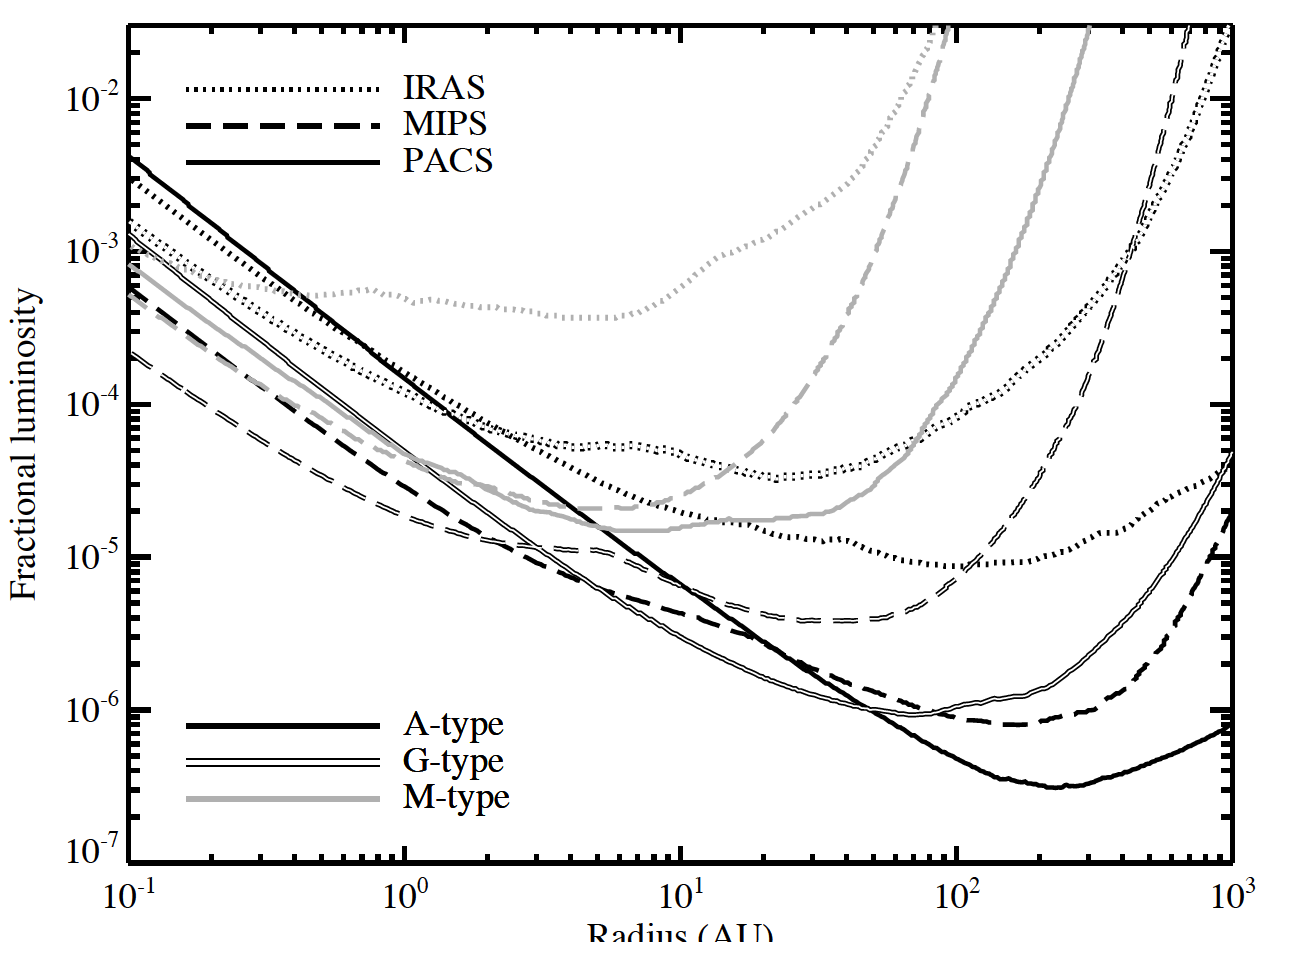
\includegraphics[scale=0.2]{Ch2/Detection_limits_Kennedy} &
    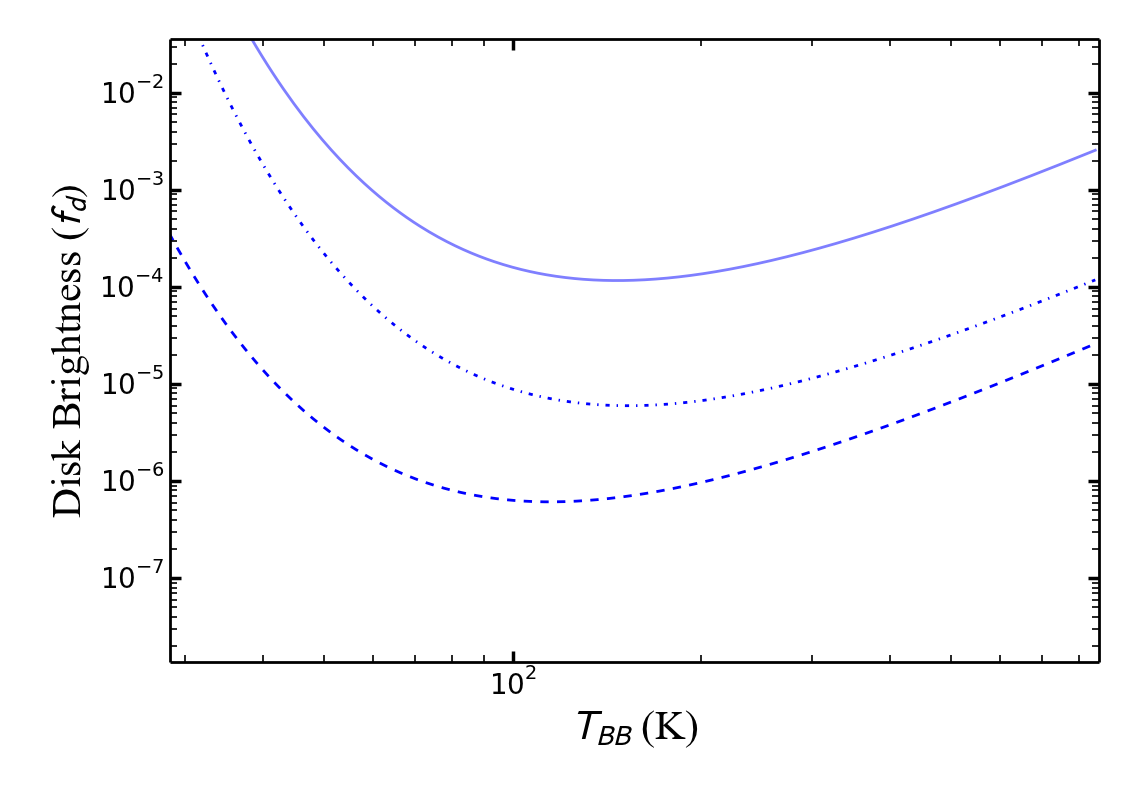
\includegraphics[scale=0.3]{Ch2/fd_vs_tbb_simple}
    \end{tabular}
    \caption[]{}
    \label{fig:detection_limits}
    \end{figure}
    %===================================================================
    
   
   The left panel of Figure~\ref{fig:detection_limits} shows the limiting fractional luminosity a few different surveys as a function of radius from the star. From IRAS to Herschel, improvements in both detector technology and an increase in mirror size have pushed the limits of detecting fainter and fainter dust populations. Hence, the increase of incidence rates from IRAS to Spitzer does not come as much of a surprise given that Spitzer is sensitive to fainter dust (cold or warm). Differences in incidence rates can also arise due to the threshold of an excess some studies may adopt compared to others. 
   
   As explained in \S~\ref{sec:excess_resolvedimaging}, the excess flux is measured from the measured IR flux subtracted from the photospheric flux in the IR, which is extrapolated from model fits to optical and near-IR flux measurements. Studies may determine the significance of an excess detection from this subtraction on a case by case basis, or from the statistical significance based on the distribution of a large survey. The former method can under or overestimate the excess if significant flux variations occur between the epoch of observations between the optical data and the IR data, while the latter technique may introduce large false-discovery rates \textbf{check this} as well as reduce the sensitivity of fainter disks for small samples in a survey. 
   
   Studies that used some of the more notable space based observatories like Herschel or Spitzer were limited to sample sizes of $\sim$500 stars, due to the pointed nature of the satellite. And although IRAS was an all-sky mission, it also produced a couple hundred excess sources. The study by \citet{Rhee2007} searched for excesses around tens of thousands of Hipparcos main-sequence stars, and produced roughly 50 new excesses, the majority of which were still cold disk detections. We have seen that cold dust is easier to detect due to the large contrast with the photosphere in the far-IR. The contrast becomes an issue in the mid-IR, where there are a relatively low number of warm dust detections.
   
   The reason behind the overall low number of warm dust detections is because of the small coverage of very sensitive pointed satellites like Spitzer and Herschel, and the relatively low resolution and sensitivity of the last all-sky mission, IRAS, where the resolution of the IRAS beam was 30'' at 12\micron. Thus, to addresss the limitations presented, I now shift focus of this thesis to finding warm dust with the latest all-sky infrared mission: the Wide-Field Infrared Survey Explorer Spacecraft.
   
   
\section{The Wide-Field Infrared Survey Explorer\\ Mission}\label{sec:wise_intro}

    The success of the IRAS mission was one of the motivations for launching another new and improved infrared all-sky mission. The goals of the Wide-Field Infrared Survey Explorer mission \citep[WISE;][]{Wright2010} were to observe the entire sky at two near-IR and two mid-IR wavelengths, thus improving and complementing the achievements of IRAS. In this section, I discuss the details of the WISE mission. Data from the WISE survey constitutes the bulk of my thesis and in the the following section, I will summarize this space based mission, its purpose and the specifications and how its data products can be used to identify circumstellar dust.
   

    \subsection{Mission Overview}\label{sec:wise_overview}


    WISE is an Earth orbiting observatory, 525~km above the Earth's surface. WISE was funded by NASA/JPL and launched on December 14th, 2009. It is a medium-class explorer mission weighing 750~kg. The satellite consists of a 40~cm diameter telescope and four imaging CCDs which are cooled by solid hydrogen cryostats. Two of the CCDs are designed to image the sky in the near-infrared wavelengths (3.5\micron and 4.6\micron) and two in the mid-infrared (12\micron and 22\micron). Figure~\ref{fig:WISE_satellite} shows an illustration of the physical satellite. 
  
    
    %===================================================================
    %  WISE SATELLITE
    %===================================================================
    \begin{figure}
    \centering
    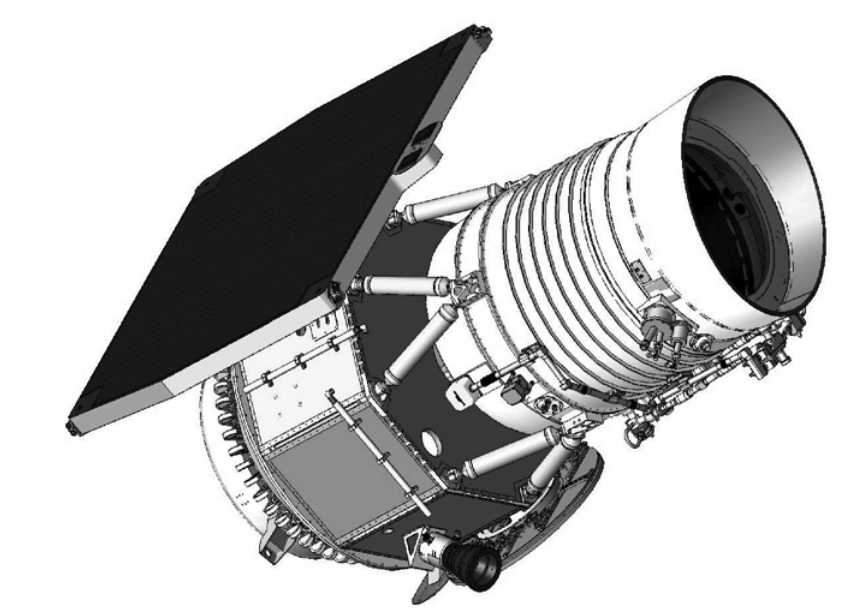
\includegraphics[width=\textwidth]{Ch2/wise_satellite}
    \caption[]{}
    \label{fig:WISE_Satellite}
    \end{figure}
    %===================================================================
    
 
    The mission was successful in scanning 99.99\% of the entire sky in the aforementioned IR bands. WISE's detector field-of-view is 47' on a side. During its continual orbit around the Earth, overlapping observation frames 11 second cadences were taken (8.8~s of integration). The overlap of frames, over multiple orbits, ensures greater depth of coverage. In a day, the satellite performs 15 orbits. Figure~\ref{fig:scan_plan} shows the overlapping frames as the satellite orbits the Earth. Further details of the entire mission can be found online\footnote{\url{http://wise2.ipac.caltech.edu/docs/release/allsky/expsup/}} or in \citet{Wright2010}. 

    %===================================================================
    %  WISE SCAN PLAN
    %===================================================================
    \begin{figure}
    \centering
    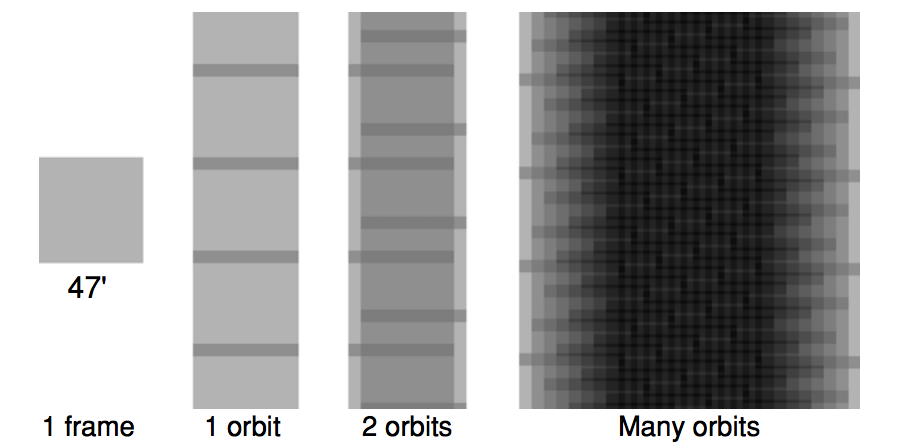
\includegraphics[width=\textwidth]{Ch2/wise_scan_plan}
    \caption[]{}
    \label{fig:wise_scan_plan}
    \end{figure}
    %===================================================================
    
    
   
   
    \subsection{WISE Bands}\label{sec:wise_bands}
   
   
   The two near-IR channels image the sky at band centered wavelengths of 3.4\micron\ and 4.6\micron\ using HgCdTe arrays, each with 18\micron\ 1024 $\times$ 1024 pixels. Both of these detectors are cooled to 32~K. The mid-IR channel detectors image the sky at band centered wavelengths of 12\micron\ and 22\micron\ and are made from Si:As BIB arrays of the same structure as the near-IR channels. These arrays are cooled to a temperature of 8.2~K. For the remainder of this thesis, I will refer to each of these bands as $W1$ (3.4\micron), $W2$ (4.6\micron), $W3$ (12\micron) and $W4$ (22\micron). Figure~\ref{fig:wise_bands} shows the relative spectral response of each of the detectors. 
   
    %===================================================================
    %  WISE BANDS
    %===================================================================
    \begin{figure}
    \centering
    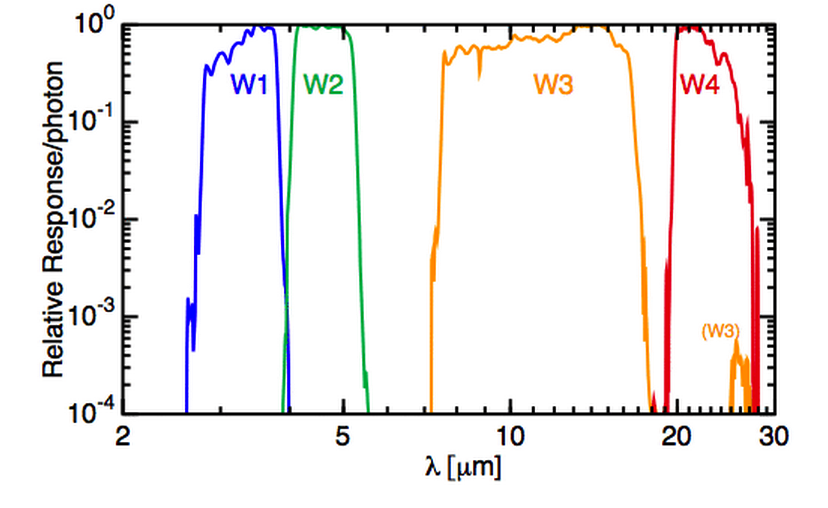
\includegraphics[scale=0.5]{Ch2/wise_response}
    \caption[]{}
    \label{fig:wise_bands}
    \end{figure}
    %===================================================================
    
    
   
    \subsection{WISE Data Products and the All-Sky Data Release}

    The WISE mission has produced a number of different data releases. The first release, called the \textit{WISE Preliminary Release} was made public on April 14, 2011\footnote{\url{http://wise2.ipac.caltech.edu/docs/release/prelim/preview.html}} and contained data that covered only 57\% of the sky. The next public release of WISE data was made on March 14, 2012. This data set was called the \textit{All-Sky Data Release}\footnote{\url{http://wise2.ipac.caltech.edu/docs/release/allsky/}} and covered the entire sky in all four bands. After the cryostats were depleted, WISE began its ``warm'' mission, and only collected data in the two near-IR $W1$ and $W2$ bands. This commenced the Near-Earth Object WISE (NEOWISE) mission. A subsequent all-sky data release by WISE came on November 13, 2013 called the \textit{All-WISE Data Release}\footnote{\url{http://wise2.ipac.caltech.edu/docs/release/allwise/}}. For the work I present in the rest of this dissertation, I only use measurements from the \textit{All-Sky Data Release}, except in comparison with other release. 
    
    Since the WISE data is in the public domain, it can easily be accessed online. The online databases consists of measurements for over half a billion objects in all four bands. These measurements consist of photometric data for each band, as well as meta-data pertaining to the quality of the data product. The database also consists of Atlas images of the processed data and can be viewed at \url{http://irsa.ipac.caltech.edu/applications/wise/}. 
    



    \subsection{Advantages Over Previous Debris Disk Surveys}

    As outlined in \S~\ref{sec:excess_resolvedimaging}, the search for an infrared excess requires precise and accurate measurement of the photospheric flux, an instrument which is sensitive to low levels of dust which is common for most debris disks ($f_\rm{d}\sim10^{-2}$), as well as the ability to discern whether the IR source detected is stellar or chance alignment. Otherwise
    
    
    The past debris disk surveys have quite well established the frequency of disks. For young stars, this incidence is relatively high ($\sim$50\% in some age groups), but as low as 20\%--30\% for intermediate mature stars for cold disk detections and as low as a few percent for warm disk incidences. Thus, identification of a large number of sources requi

    
    %===================================================================
    %  Mission Sensitivities
    %===================================================================
    \begin{figure}
    \centering
    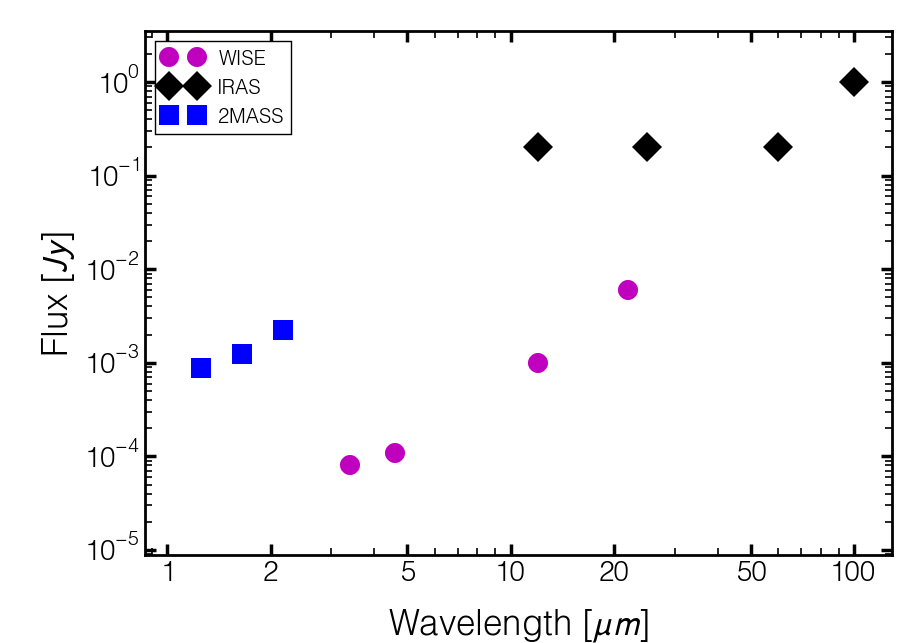
\includegraphics[scale=0.5]{Ch2/flux_density_comparison}
    \caption[]{}
    \label{fig:flux_comparison}
    \end{figure}
    %===================================================================
    
    
    
    
    
    
    %===================================================================
    %  IRAS vs. WISE
    %===================================================================
    %\begin{figure}
    %\centering
    %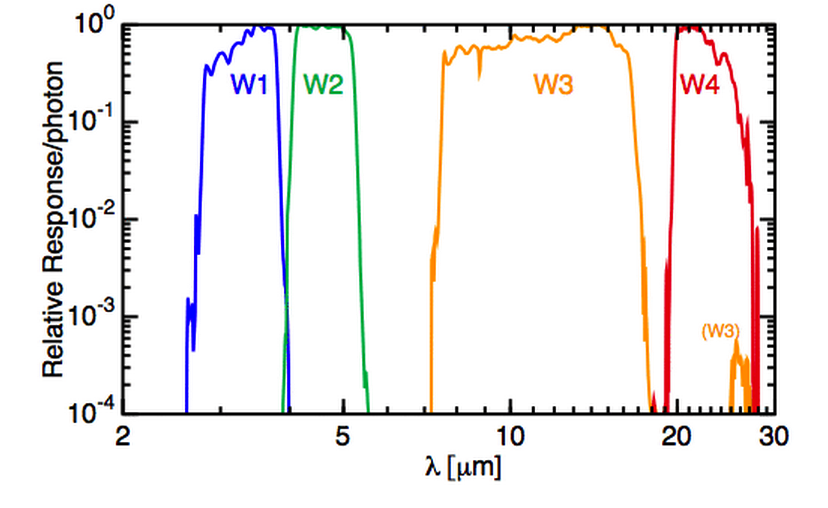
\includegraphics[scale=0.5]{Ch2/wise_response}
    %\caption[]{}
    %\label{fig:wise_bands}
    %\end{figure}
    %===================================================================
    
    
\clearpage
%\setboolean{@twoside}{false}
%\includepdf[pages=-,offset=75 -75]{Ch2/WISEPaper_PMH14.pdf}


\chapter{Confirming Excesses Through Weighted Combination of Colors}\label{chap:confirm}

\chapter{120 pc Volume Disk Analysis}

\chapter{Summary of Results}\label{chap:summary}

\chapter{Discussion}\label{chap:discussion}

\chapter{Summary and Future Direction} \label{chap:future}




%\include{ch1_introduction}


%\include{chapter2}
% ...

%%%%%%%%%%%%%%%%%%%%%%%%%%%%%%%%%%%%%%%%%%%%%%%%%%%%%%%%%%%%%%%%%%%%%%%%%%%%%%%%

%\appendix

%\include{appendix1}
%\include{appendix2}
% ...

%%%%%%%%%%%%%%%%%%%%%%%%%%%%%%%%%%%%%%%%%%%%%%%%%%%%%%%%%%%%%%%%%%%%%%%%%%%%%%%%

\bibliography{References_PhD}
\end{document}